\documentclass[UTF8,aspectratio=169]{beamer}



% 基本包
\usepackage[UTF8]{ctex}
\usepackage{graphicx}
\usepackage{amsmath}
\usepackage{amsfonts}
\usepackage{amssymb}
% \usepackage{listings}  % 已替换为minted
\usepackage{xcolor}
\usepackage{hyperref}
\usepackage{booktabs}
\usepackage{multirow}
\usepackage{multicol}
\usepackage{float}
\usepackage{tikz}
\usetikzlibrary{positioning,shapes,arrows,fit,backgrounds}
\usepackage{pgfplots}
\pgfplotsset{compat=1.18}
\usepackage{minted}
\usepackage{fontspec}
\usepackage[most]{tcolorbox}

% Beamer主题设置
\usetheme{Madrid}
\usecolortheme{whale}

% 校徽设置
\logo{
  \IfFileExists{../长江大学校徽.pdf}{
    \begin{tikzpicture}[remember picture,overlay]
      \node[anchor=north east, xshift=-0.2mm, yshift=-0.2mm] at (current page.north east) {
        
\includegraphics[height=1.0cm]{../长江大学校徽.pdf}
      };
    \end{tikzpicture}
  }{
    \begin{tikzpicture}[remember picture,overlay]
      \node[anchor=north east, xshift=-3mm, yshift=-3mm] at (current page.north east) {
        \textcolor{red}{\tiny []}
      };
    \end{tikzpicture}
  }
}

% ===== 使用推荐的 font themes =====
\usefonttheme{professionalfonts}  % 允许自定义字体

% 自定义frame标题栏,也缩短长度留出logo空间
% 设置标题栏背景颜色为淡蓝色
\definecolor{frametitlebg}{RGB}{200,215,250} % 淡蓝色,可根据需要调整
\setbeamercolor{frametitle}{bg=frametitlebg, fg=ytublue!80!black}
\setbeamertemplate{frametitle}{
  \ifbeamercolorempty[bg]{frametitle}{}{\nointerlineskip}%
  \begin{tcolorbox}[
    enhanced,
    width=0.90\paperwidth,
    height=2.5ex,
    colback=frametitlebg,
    colframe=frametitlebg,
    boxrule=0pt,
    left=0pt,
    right=0pt,
    top=1pt,
    bottom=0pt,
    boxsep=0pt,
    before skip=0pt,
    after skip=0.1em,  % 减少标题栏和内容之间的间距
  ]
  \vspace{0.2ex} % 减少标题文字上方的空白
  \usebeamerfont{frametitle}\textcolor{ytublue!80!black}{\hspace{1em}\insertframetitle}
  \end{tcolorbox}
}

% ===== 设置现代字体 =====
\setsansfont{Source Sans Pro}     % 正文字体
\setmonofont{Source Code Pro}[Scale=0.9]  % 代码字体,稍微缩小一点

\setbeamertemplate{navigation symbols}{}

% 减少页面间距
\setbeamertemplate{itemize items}[circle]
\setbeamertemplate{enumerate items}[default]
\setlength{\itemsep}{0.1em}
\setlength{\parskip}{0.1em}

% 页码设置
\setbeamertemplate{footline}[frame number]

% 定义流程图样式
\tikzset{
    block/.style = {rectangle, draw, fill=blue!10,
        minimum width=6em, align=center, rounded corners, minimum height=3em},
    line/.style = {draw, -latex'}
}
% 水印设置
\setbeamertemplate{background}{
    \begin{tikzpicture}[remember picture,overlay]
        \node[rotate=-45,scale=0.8,opacity=0.1,color=gray]
             at ([xshift=0.5cm,yshift=0.5cm]current page.south west)
             {\large\textbf{WPJ}};
    \end{tikzpicture}
}

% 自定义颜色
\definecolor{qtgreen}{RGB}{41,128,185}
\definecolor{qtblue}{RGB}{52,73,94}

% 定义长江大学蓝主色调
\definecolor{ytublue}{RGB}{0,84,159}
% 统一block样式
\newtcolorbox{ytublock}[1]{
  colback=white,
  colframe=ytublue!80!black,
  colbacktitle=ytublue!20!white,
  coltitle=ytublue!80!black,
  title={#1},
  fonttitle=\bfseries,
  arc=3mm,
  boxrule=1pt,
  boxsep=1mm,
  left=2mm,
  right=2mm,
  top=0.5mm,
  bottom=0.5mm,
  before skip=3pt,
  after skip=3pt,
  enhanced,
  drop fuzzy shadow=ytublue!20!black
}

% 定义警告块样式
\newtcolorbox{ytualertblock}[1]{
  colback=white,
  colframe=red!80!black,
  colbacktitle=red!20!white,
  coltitle=red!80!black,
  title={#1},
  fonttitle=\bfseries,
  arc=3mm,
  boxrule=1.5pt,
  boxsep=1mm,
  left=2mm,
  right=2mm,
  top=0.5mm,
  bottom=0.5mm,
  before skip=3pt,
  after skip=3pt,
  enhanced,
  drop fuzzy shadow=red!20!black,
  overlay={
    \begin{tcbclipinterior}
      \fill[red!10!white] (interior.south west) rectangle (interior.north east);
    \end{tcbclipinterior}
  }
}

% cpp代码高亮设置
\setminted[cpp]{
    fontsize=\tiny,
    fontfamily=tt,             % 使用等宽字体
    linenos=true,
    frame=lines,               % 上下两条线,简洁清爽(比 tb 更现代)
    framesep=3mm,              % 内边距
    rulecolor=\color{blue!20}, % 线条颜色浅蓝,不刺眼
    bgcolor=blue!10,           % 浅蓝色背景
    baselinestretch=1.2,       % 行距稍大,更易读
    breaklines=true,
    breakautoindent=true,
    tabsize=4,
    xleftmargin=5mm,
    xrightmargin=5mm,
    numbersep=8pt,             % 行号与代码间距
    % ===== 其他美化 =====
    obeytabs=true,             % 尊重 tab 字符
    samepage=false,            % 允许跨页(重要!避免空白)
    escapeinside=||,           % 可在代码中使用 |LaTeX| 插入 LaTeX 命令
}

% 设置标题页颜色,与frame标题保持一致
\setbeamercolor{title}{bg=frametitlebg, fg=ytublue!80!black}
\setbeamercolor{subtitle}{bg=frametitlebg, fg=ytublue!70!black}
\setbeamercolor{author}{bg=frametitlebg, fg=ytublue!80!black}
\setbeamercolor{institute}{bg=frametitlebg, fg=ytublue!80!black}
\setbeamercolor{date}{bg=frametitlebg, fg=ytublue!80!black}

% 自定义标题页样式,全部内容同一个tcolorbox,居中排版,字体和间距区分
\setbeamertemplate{title page}{
  \vbox{}
  \begingroup
    \centering
    \begin{tcolorbox}[
      enhanced,
      width=0.92\paperwidth,
      colback=frametitlebg,
      colframe=frametitlebg,
      boxrule=0pt,
      left=0pt,
      right=0pt,
      top=4mm,
      bottom=4mm,
      boxsep=0pt,
      before skip=0pt,
      after skip=1.2em,
    ]
    % 标题
    {\centering
      {\fontsize{24pt}{27pt}\selectfont\textcolor{ytublue!80!black}{\inserttitle}\par}
      \vspace{1.2em}
      % 副标题
      {\fontsize{21pt}{24pt}\selectfont\textcolor{ytublue!70!black}{\insertsubtitle}\par}
      \vspace{2.0em}
      % 作者
      {\fontsize{12pt}{15pt}\selectfont\insertauthor\par}
      \vspace{0.7em}
      % 单位
      {\fontsize{12pt}{15pt}\selectfont\insertinstitute\par}
      \vspace{0.7em}
      % 日期
      {\fontsize{12pt}{15pt}\selectfont\insertdate\par}
    }
    \vspace{0.5em}
    \vfill
    \end{tcolorbox}
  \endgroup
}


% 文档信息
\title{高等程序设计 - Qt/C++}
\subtitle{第5章:设计模式}
\author{王培杰}
\institute{长江大学地球物理与石油资源学院}
\date{\today}


\begin{document}

% 标题页
\begin{frame}
    \titlepage
\end{frame}

% 目录页
\begin{frame}{目录}
    \begin{multicols}{2}
        \tableofcontents[hideothersubsections]
    \end{multicols}
\end{frame}

\section{设计模式概述}
\begin{frame}{目录}
    \begin{multicols}{2}
        \tableofcontents[currentsection,hideothersubsections]
    \end{multicols}
\end{frame}

\begin{frame}{设计模式概述}
    \begin{ytublock}{什么是设计模式}
        \begin{itemize}
            \item 设计模式(Design Pattern)是前人总结出的、在软件开发中反复出现的、行之有效的代码结构和解决方案。
            \item GoF 在其经典著作《设计模式:可复用面向对象软件的基础》中,将设计模式分为三大类:创建型模式、结构型模式和行为型模式,共\textbf{23种经典模式}。
            \item 设计模式不是具体的代码实现,而是一种可复用的设计思想和最佳实践,帮助开发者解决常见的软件设计问题。
            \item 设计模式提高了代码的可维护性、可扩展性和复用性,促进团队协作和沟通。
            \item 学习和应用设计模式有助于理解面向对象设计原则,提升软件架构能力。
            \item 设计模式是软件工程的基石,是软件开发中不可或缺的重要知识。
        \end{itemize}
    \end{ytublock}
\end{frame}

\begin{frame}{23种GoF设计模式分类}
    \begin{columns}
        \begin{column}{0.32\textwidth}
            \begin{ytublock}{创建型模式 (5种)}
                \begin{itemize}
                    \item \textbf{单例模式}
                    \item \textbf{工厂方法}
                    \item \textbf{抽象工厂}
                    \item \textbf{建造者模式}
                    \item \textbf{原型模式}
                \end{itemize}
            \end{ytublock}
        \end{column}
        \begin{column}{0.32\textwidth}
            \begin{ytublock}{结构型模式 (7种)}
                \begin{itemize}
                    \item \textbf{适配器模式}
                    \item \textbf{桥接模式}
                    \item \textbf{组合模式}
                    \item \textbf{装饰器模式}
                    \item \textbf{外观模式}
                    \item \textbf{享元模式}
                    \item \textbf{代理模式}
                \end{itemize}
            \end{ytublock}
        \end{column}
        \begin{column}{0.32\textwidth}
            \begin{ytublock}{行为型模式 (11种)}
                \begin{itemize}
                    \item \textbf{责任链模式}
                    \item \textbf{命令模式}
                    \item \textbf{解释器模式}
                    \item \textbf{迭代器模式}
                    \item \textbf{中介者模式}
                    \item \textbf{备忘录模式}
                    \item \textbf{观察者模式}
                    \item \textbf{状态模式}
                    \item \textbf{策略模式}
                    \item \textbf{模板方法}
                    \item \textbf{访问者模式}
                \end{itemize}
            \end{ytublock}
        \end{column}
    \end{columns}
\end{frame}

\section{创建型模式}
\begin{frame}{目录}
    \begin{multicols}{2}
        \tableofcontents[currentsection,hideothersubsections]
    \end{multicols}
\end{frame}

\begin{frame}{创建型模式(Creational Patterns)}
    \begin{ytublock}{什么是创建型模式}
        创建型模式其实就是帮我们"怎么创建对象更灵活"。
        如果我们直接用 \texttt{new} 去创建对象,代码会和具体的类绑死,后期想改、想扩展都很麻烦。

        创建型模式就是用一些通用套路,把"怎么创建对象"这件事封装起来,让我们不用关心细节,想换对象、加功能都很方便。
        这样代码更容易维护,也更容易扩展。

        这些模式可以让我们按需选择、组合、甚至复用对象,适应各种实际开发场景。

        常见的创建型模式有:单例模式(全局唯一对象)、
        工厂方法模式(延迟决定创建哪种对象)、
        抽象工厂模式(创建一组相关对象)、
        建造者模式(一步步构建复杂对象)、
        原型模式(通过克隆快速生成新对象)等。
        每种模式都有自己的用武之地,比如只要一个实例、需要一组产品、对象很复杂、或者需要大量相似对象时,都能用上。
    \end{ytublock}
\end{frame}

\begin{frame}{创建型模式}
    \begin{ytublock}{创建型模式}
        创建型模式(Creational Patterns)专注于如何高效、灵活、可控地创建对象。它们将对象的创建与使用解耦,隐藏了实例化的具体细节,便于系统在不影响已有代码的情况下引入新的对象类型。常见的创建型模式包括:
        \begin{itemize}
            \item \textbf{单例模式(Singleton Pattern)}:保证一个类只有一个实例,并提供全局访问点。常用于全局配置、日志管理等场景。
            \item \textbf{工厂方法模式(Factory Method Pattern)}:定义一个用于创建对象的接口,让子类决定实例化哪一个类。适用于需要将对象的创建延迟到子类的情况。
            \item \textbf{抽象工厂模式(Abstract Factory Pattern)}:提供一个创建一系列相关或相互依赖对象的接口,而无需指定它们具体的类。适合产品族的创建。
            \item \textbf{建造者模式(Builder Pattern)}:将一个复杂对象的构建与它的表示分离,使同样的构建过程可以创建不同的表示。常用于复杂对象的分步构建。
            \item \textbf{原型模式(Prototype Pattern)}:通过复制已有实例来创建新对象,而不是通过 new 关键字。适合对象创建成本较高或需要大量相似对象的场景。
        \end{itemize}
    \end{ytublock}
\end{frame}

\subsection{单例模式(Singleton Pattern)}

\begin{frame}{单例模式(Singleton Pattern)}
    保证一个类仅有一个实例,并提供一个访问它的全局访问点。
    \begin{ytublock}{适用场景}
        \begin{itemize}
            \item 当类只能有一个实例而且客户可以从一个众所周知的访问点访问它时。
            \item 当这个唯一实例应该是通过子类化可扩展的,并且客户应该无需更改代码就能使用一个扩展的实例时。
        \end{itemize}
    \end{ytublock}
    \begin{columns}
        \begin{column}{0.30\textwidth}
            \begin{ytublock}{例如:全局配置}
                \begin{itemize}
                    \item 配置管理器
                    \item 日志管理器
                    \item 数据库管理器
                    \item 线程池管理器
                    \item 缓存管理器
                \end{itemize}
            \end{ytublock}
        \end{column}
        \begin{column}{0.68\textwidth}
            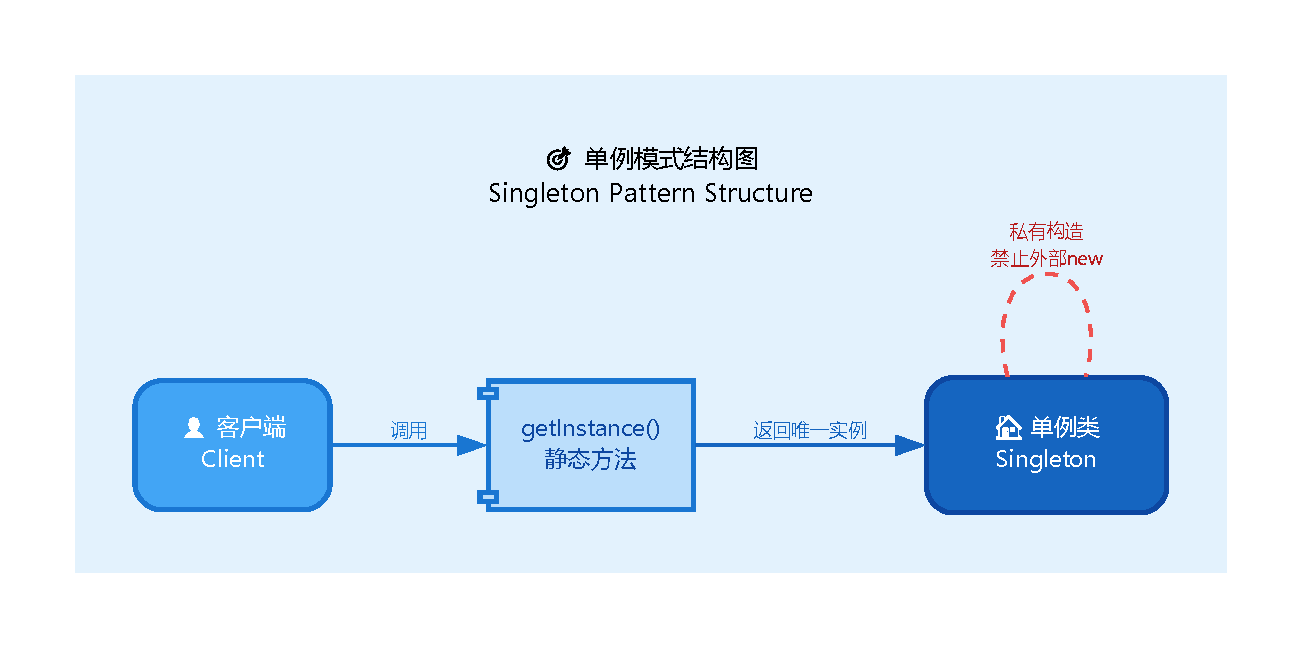
\includegraphics[width=1.0\textwidth]{images/singleton_pattern.pdf}
        \end{column}
    \end{columns}
\end{frame}

\begin{frame}{单例模式举例说明}
    \begin{exampleytublock}{打印机管理系统——单例模式}
        假设我们要开发一个打印机管理系统,要求全局只存在一个打印队列管理器,所有用户和程序都通过它来提交打印任务,避免多台打印机同时混乱工作。
        \textbf{单例模式}的做法是:
        \begin{itemize}
            \item 首先定义一个打印队列管理器类(\texttt{PrinterManager}),用于统一管理所有的打印任务。
            \item 将\texttt{PrinterManager}设计为单例类,确保全局只有一个实例,并提供静态方法获取该实例。
            \item 程序的各个部分都通过该单例对象提交打印任务,保证打印任务的有序和统一管理。
        \end{itemize}
    \end{exampleytublock}
\end{frame}

\begin{frame}{单例模式类型}
    \begin{columns}
        \begin{column}{0.32\textwidth}
            \textbf{饿汉式单例模式}:\\
            在程序启动或类加载时立即创建唯一实例。\\
            \textbf{优点}:实现简单,天然线程安全。\\
            \textbf{缺点}:如果实例创建开销较大且未必用到,可能造成资源浪费。\\
            \textbf{适用场景}:实例始终会被使用。
        \end{column}
        \begin{column}{0.32\textwidth}
            \textbf{懒汉式单例模式}:\\
            在第一次使用时才创建实例。\\
            \textbf{优点}:按需分配资源,避免不必要的资源浪费。\\
            \textbf{缺点}:多线程下实现复杂,需加锁保证线程安全。\\
            \textbf{适用场景}:实例可能不会被使用。
        \end{column}
        \begin{column}{0.32\textwidth}
            \textbf{静态局部变量单例(C++11推荐)}:\\
            利用函数内静态局部变量特性,首次调用时创建实例,C++11后线程安全。\\
            \textbf{优点}:懒加载,线程安全,代码简洁。\\
            \textbf{缺点}:依赖编译器对C++11标准的支持。\\
            \textbf{适用场景}:推荐C++实现单例时使用。
        \end{column}
    \end{columns}
\end{frame}

\begin{frame}{单例模式示例——饿汉式}
    \begin{columns}
        \begin{column}{0.48\textwidth}
            \inputminted[firstline=7, lastline=22]{cpp}{code/singleton_pattern.cpp}
        \end{column}
        \begin{column}{0.48\textwidth}
            \inputminted[firstline=23, lastline=38]{cpp}{code/singleton_pattern.cpp}
        \end{column}
    \end{columns}
\end{frame}

\begin{frame}{单例模式示例——懒汉式}
    \begin{columns}
        \begin{column}{0.48\textwidth}
            \inputminted[firstline=40, lastline=59]{cpp}{code/singleton_pattern.cpp}
        \end{column}
        \begin{column}{0.48\textwidth}
            \inputminted[firstline=60, lastline=78]{cpp}{code/singleton_pattern.cpp}
        \end{column}
    \end{columns}
\end{frame}

\begin{frame}{单例模式示例——静态内部类}
    \begin{columns}
        \begin{column}{0.48\textwidth}
            \inputminted[firstline=80, lastline=96]{cpp}{code/singleton_pattern.cpp}
        \end{column}
        \begin{column}{0.48\textwidth}
            \inputminted[firstline=97, lastline=112]{cpp}{code/singleton_pattern.cpp}
        \end{column}
    \end{columns}
\end{frame}

\begin{frame}{单例模式使用}
    \begin{columns}
        \begin{column}{0.48\textwidth}
            \inputminted[firstline=120, lastline=135]{cpp}{code/singleton_pattern.cpp}
        \end{column}
        \begin{column}{0.48\textwidth}
            \inputminted[firstline=136, lastline=152]{cpp}{code/singleton_pattern.cpp}
        \end{column}
    \end{columns}
\end{frame}

\begin{frame}{单例模式优缺点}
    \begin{ytublock}{优点}
        \begin{itemize}
            \item 全局唯一实例,节省内存,便于统一管理资源
            \item 避免频繁创建和销毁实例,减少系统开销
            \item 提高系统性能,适合需要频繁访问的共享资源
            \item 提供全局访问点,方便在系统各处获取实例
            \item 可以延迟实例化(懒汉式),按需分配资源
        \end{itemize}
    \end{ytublock}
    \begin{alertytublock}{缺点}
        \begin{itemize}
            \item 不利于单元测试,难以模拟和替换单例对象
            \item 可能隐藏依赖关系,增加代码耦合
            \item 多线程环境下实现复杂,容易引发线程安全问题
            \item 滥用单例会导致"伪全局变量",影响系统扩展性
            \item 生命周期与程序一致,可能导致资源无法及时释放
        \end{itemize}
    \end{alertytublock}
\end{frame}

\subsection{工厂方法模式(Factory Method Pattern)}

\begin{frame}{工厂方法模式(Factory Method Pattern)}
    工厂方法模式(Factory Method Pattern)是一种创建型设计模式。它定义了一个用于创建对象的接口,但由子类决定要实例化的具体类。工厂方法使一个类的实例化延迟到其子类。
    \begin{ytublock}{适用场景}
        \begin{itemize}
            \item 当一个类不知道它所必须创建的对象的类时。
            \item 当一个类希望由它的子类来指定它所创建的对象时。
            \item 当类将创建对象的职责委托给多个帮助子类中的某一个,并且你希望将哪一个帮助子类是代理者这一信息局部化时。
            \item 需要灵活切换产品系列,或系统中产品类型经常变化时。
        \end{itemize}
    \end{ytublock}
\end{frame}

\begin{frame}{工厂方法模式结构}
    \begin{columns}
        \begin{column}{0.48\textwidth}
            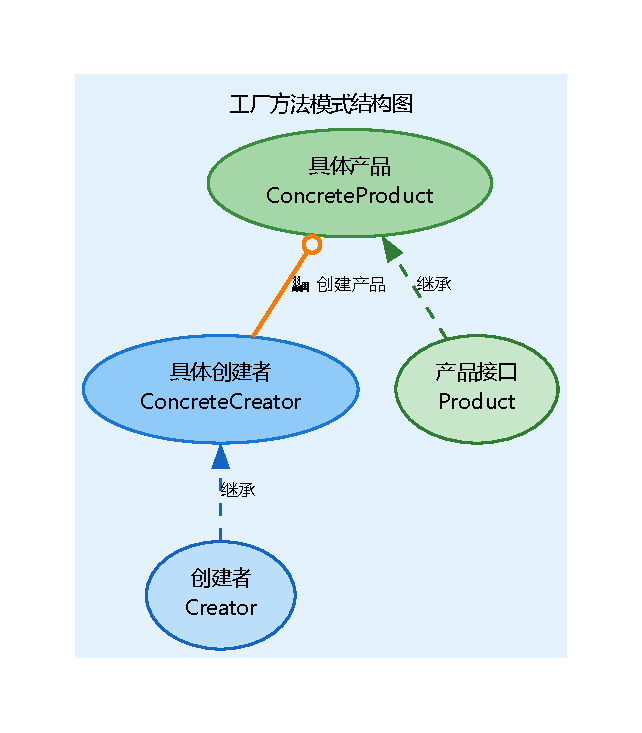
\includegraphics[width=1.0\textwidth]{images/factory_method_pattern.pdf}
        \end{column}
        \begin{column}{0.48\textwidth}
            \begin{ytublock}{结构}
                工厂方法模式主要包含以下角色:
                \begin{itemize}
                    \item \textbf{抽象产品(Product)}:定义产品的规范,描述产品的主要特性和功能。
                    \item \textbf{具体产品(ConcreteProduct)}:实现抽象产品接口,定义具体的产品对象。
                    \item \textbf{抽象工厂(Creator)}:声明工厂方法,用于返回一个产品对象。可以定义一个工厂方法的默认实现,返回默认的产品对象。
                    \item \textbf{具体工厂(ConcreteCreator)}:重写工厂方法,返回具体的产品实例。
                \end{itemize}
            \end{ytublock}
        \end{column}
    \end{columns}
\end{frame}

\begin{frame}{工厂方法模式举例}
    \begin{exampleytublock}{饮料工厂——工厂方法模式}
        假设我们要开发一个饮料工厂,能够根据不同的需求生产不同类型的饮料(如可乐、果汁、茶等)。
        \textbf{工厂方法模式}的做法是:
        \begin{itemize}
            \item 首先定义一个饮料产品的抽象类(\texttt{Beverage}),所有饮料都继承自它。
            \item 再定义一个工厂的抽象类(\texttt{BeverageFactory}),其中声明一个生产饮料的工厂方法(如\texttt{createBeverage()})。
            \item 每种具体饮料(如\texttt{Cola}、\texttt{Juice}、\texttt{Tea})都实现\texttt{Beverage}类。
            \item 每种具体饮料工厂(如\texttt{ColaFactory}、\texttt{JuiceFactory}、\texttt{TeaFactory})都继承自\texttt{BeverageFactory},并实现\texttt{createBeverage()}方法,负责生产对应的饮料对象。
        \end{itemize}
        \vspace{0.5em}
        \textbf{优点:} 客户端只需与工厂接口和产品接口打交道,无需关心具体产品的创建细节,便于扩展和维护。
    \end{exampleytublock}
\end{frame}

\begin{frame}{工厂方法模式示例(一)}
    \begin{columns}
        \begin{column}{0.48\textwidth}
            \inputminted[firstline=1, lastline=19]{cpp}{code/factory_method_pattern.cpp}
        \end{column}
        \begin{column}{0.48\textwidth}
            \inputminted[firstline=20, lastline=38]{cpp}{code/factory_method_pattern.cpp}
        \end{column}
    \end{columns}
\end{frame}

\begin{frame}{工厂方法模式示例(二)}
    \begin{columns}
        \begin{column}{0.48\textwidth}
            \inputminted[firstline=40, lastline=55]{cpp}{code/factory_method_pattern.cpp}
        \end{column}
        \begin{column}{0.48\textwidth}
            \inputminted[firstline=56, lastline=70]{cpp}{code/factory_method_pattern.cpp}
        \end{column}
    \end{columns}
\end{frame}

\begin{frame}{工厂方法模式优缺点}
    \begin{ytublock}{优点}
        \begin{itemize}
            \item 工厂方法模式将产品创建的逻辑封装在具体工厂类中,客户端无需关心产品创建的具体过程,符合开闭原则。
            \item 通过工厂方法模式,可以灵活地添加新的产品类型,而无需修改现有的工厂类,符合开闭原则。
            \item 工厂方法模式可以更好地组织和管理产品创建的逻辑,使得代码更加清晰和易于维护。
        \end{itemize}
    \end{ytublock}
    \begin{alertytublock}{缺点}
        \begin{itemize}
            \item 工厂方法模式需要创建多个具体工厂类,增加了系统的复杂性。
            \item 工厂方法模式需要客户端知道具体工厂类的名称,增加了耦合度。
            \item 工厂方法模式需要客户端知道具体产品的名称,增加了耦合度。
        \end{itemize}
    \end{alertytublock}
\end{frame}

\subsection{抽象工厂模式(Abstract Factory Pattern)}

\begin{frame}{抽象工厂模式(Abstract Factory Pattern)}
    提供一个创建一系列相关或相互依赖对象的接口,而无需指定它们具体的类。
    \begin{ytublock}{适用场景}
        \begin{itemize}
            \item 一个系统要独立于它的产品的创建、组合和表示时。
            \item 一个系统要由多个产品系列中的一个来配置时。
            \item 当要强调一系列相关的产品对象的设计以便进行联合使用时。
            \item 当提供一个产品类库,而只想显示它们的接口而不是实现时。
        \end{itemize}
    \end{ytublock}
\end{frame}

\begin{frame}{抽象工厂模式结构}
    \begin{ytublock}{结构}
        抽象工厂模式主要包含以下角色:
        \begin{itemize}
            \item \textbf{抽象产品}:为一类产品提供统一的接口或抽象类,规定产品应有的功能。
            \item \textbf{具体产品}:实现抽象产品接口,代表实际生产的具体产品对象。
            \item \textbf{抽象工厂}:声明创建一组相关产品的接口,通常包含多个创建不同产品的方法。
            \item \textbf{具体工厂}:实现抽象工厂接口,负责实例化一组具体产品。
        \end{itemize}
    \end{ytublock}
    \begin{ytublock}{与工厂方法模式的区别}
        \begin{itemize}
            \item 工厂方法模式针对的是\textbf{一个产品等级结构},而抽象工厂模式针对的是\textbf{多个产品等级结构}(即一组产品族)。
            \item 工厂方法模式每次只生产\textbf{一种产品},而抽象工厂模式可以生产\textbf{一组相关的产品}。
            \item 工厂方法模式通常只有一个工厂接口,抽象工厂模式则包含多个产品的工厂方法。
            \item 抽象工厂模式强调产品族的约束,保证同一工厂生产的产品是相互兼容的。
        \end{itemize}
    \end{ytublock}
\end{frame}

\begin{frame}{抽象工厂模式结构}
        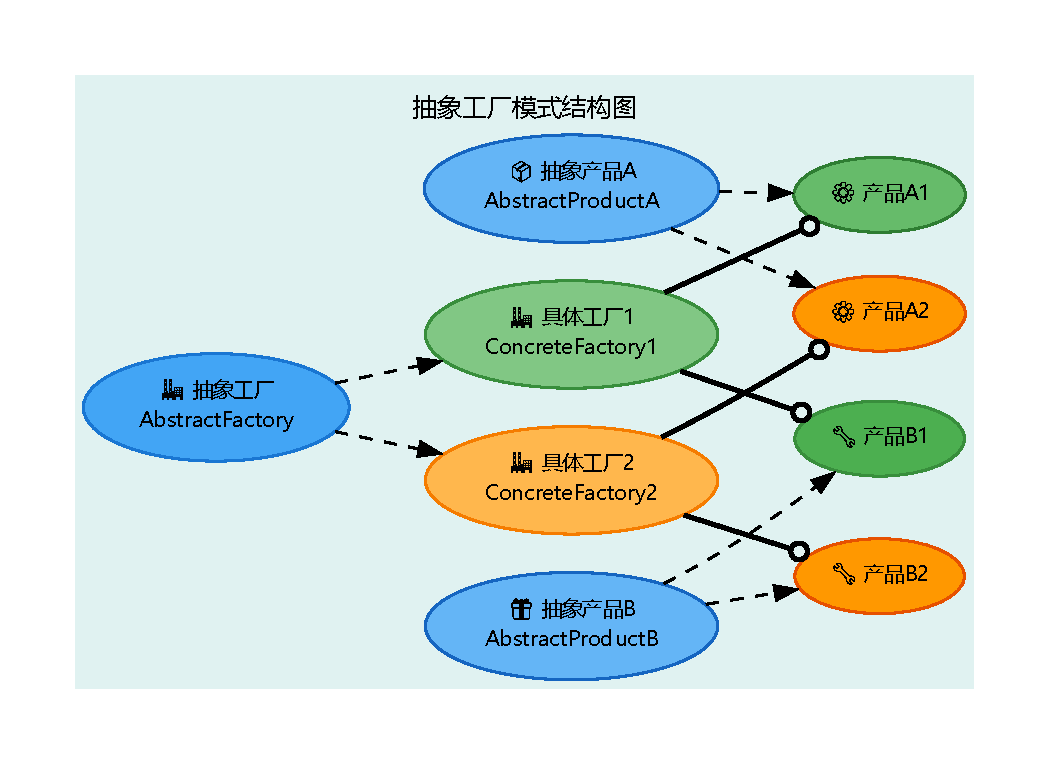
\includegraphics[width=0.8\textwidth]{images/abstract_factory_pattern.pdf}
\end{frame}

\begin{frame}{抽象工厂模式举例说明}
    \begin{exampleytublock}{奶茶店系统——抽象工厂模式}
        假设我们要开发一个奶茶店系统,奶茶店提供多种不同口味的奶茶(如\texttt{原味}、\texttt{甜味}、\texttt{巧克力味}等),以及不同的饮品配料(如\texttt{牛奶}、\texttt{糖}、\texttt{巧克力}等)。
        \textbf{抽象工厂模式}的实现思路如下:
        \begin{itemize}
            \item 定义奶茶产品的抽象类(如\texttt{Tea}),所有具体奶茶类(如\texttt{原味奶茶}、\texttt{甜味奶茶}、\texttt{巧克力味奶茶})都继承自它。
            \item 定义配料产品的抽象类(如\texttt{Topping}),所有具体配料类(如\texttt{牛奶}、\texttt{糖}、\texttt{巧克力})都继承自它。
            \item 定义抽象工厂(如\texttt{TeaFactory}),声明创建奶茶和配料的接口(如\texttt{createTea()}和\texttt{createTopping()})。
            \item 定义具体工厂(如\texttt{原味Factory}、\texttt{甜味Factory}、\texttt{巧克力味Factory}),分别实现抽象工厂接口,生产一组特定口味的奶茶和配料。
        \end{itemize}
        \textbf{优点:} 客户端只需依赖抽象工厂和产品接口,无需关心具体产品的创建细节,便于系统的扩展和维护。当需要增加新的产品族时,只需增加新的工厂类即可,无需修改已有代码。例如添加新的口味或配料,只需实现新的工厂类即可,无需修改已有代码。
    \end{exampleytublock}
\end{frame}

\begin{frame}{抽象工厂模式示例(一)}
    \begin{columns}
        \begin{column}{0.48\textwidth}
            \inputminted[firstline=1, lastline=19]{cpp}{code/abstract_factory_pattern.cpp}
        \end{column}
        \begin{column}{0.48\textwidth}
            \inputminted[firstline=21, lastline=41]{cpp}{code/abstract_factory_pattern.cpp}
        \end{column}
    \end{columns}
\end{frame}

\begin{frame}{抽象工厂模式示例(二)}
    \begin{columns}
        \begin{column}{0.48\textwidth}
            \inputminted[firstline=43, lastline=63]{cpp}{code/abstract_factory_pattern.cpp}
        \end{column}
        \begin{column}{0.48\textwidth}
            \inputminted[firstline=65, lastline=81]{cpp}{code/abstract_factory_pattern.cpp}
        \end{column}
    \end{columns}
\end{frame}

\begin{frame}{抽象工厂模式示例(三)}
    \begin{columns}
        \begin{column}{0.48\textwidth}
            \inputminted[firstline=83, lastline=102]{cpp}{code/abstract_factory_pattern.cpp}
        \end{column}
        \begin{column}{0.48\textwidth}
            \inputminted[firstline=104, lastline=124]{cpp}{code/abstract_factory_pattern.cpp}
        \end{column}
    \end{columns}
\end{frame}

\begin{frame}{抽象工厂模式优缺点}
    \begin{ytublock}{优点}
        \begin{itemize}
            \item 抽象工厂模式将产品族的创建与使用分离,符合开闭原则。
            \item 抽象工厂模式可以灵活地添加新的产品族,而无需修改现有的工厂类,符合开闭原则。
            \item 抽象工厂模式可以更好地组织和管理产品族的创建逻辑,使得代码更加清晰和易于维护。
        \end{itemize}
    \end{ytublock}
    \begin{alertytublock}{缺点}
        \begin{itemize}
            \item 抽象工厂模式需要创建多个具体工厂类,增加了系统的复杂性。
            \item 抽象工厂模式需要客户端知道具体工厂类的名称,增加了耦合度。
            \item 抽象工厂模式需要客户端知道具体产品的名称,增加了耦合度。
        \end{itemize}
    \end{alertytublock}
\end{frame}

\subsection{建造者模式(Builder Pattern)}

\begin{frame}{建造者模式(Builder Pattern)}
    \textbf{建造者模式(Builder Pattern)}是一种创建型设计模式,它将一个复杂对象的构建过程与其最终的表示分离。通过这种方式,同样的构建过程可以创建不同的产品表示。
    \begin{ytublock}{适用场景}
        \begin{itemize}
            \item 当一个对象的构建过程复杂,且需要按照特定顺序分步骤创建时。
            \item 当需要创建的产品有不同的表示(即产品的组成部件相同,但装配方式或细节不同)时。
            \item 当构建过程独立于产品的组成部分和装配方式时。
        \end{itemize}
    \end{ytublock}
\end{frame}

\begin{frame}{建造者模式结构}
    \begin{columns}
        \begin{column}{0.48\textwidth}
            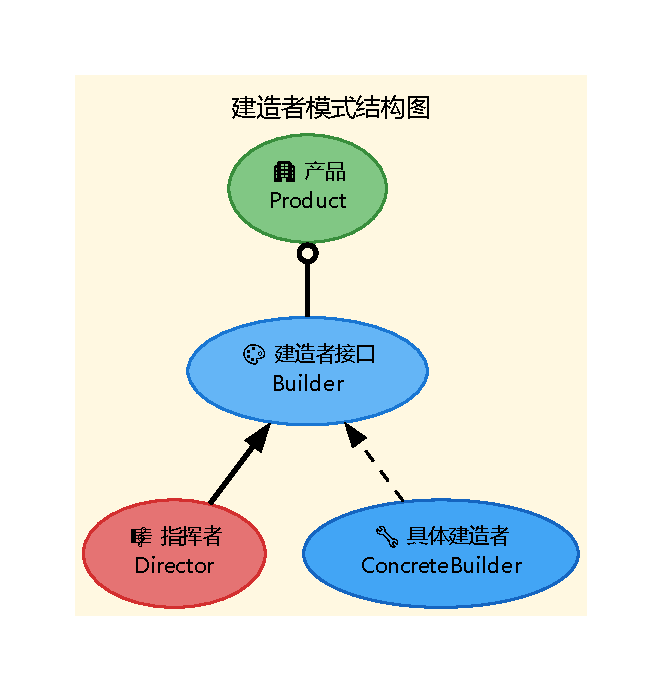
\includegraphics[width=1.0\textwidth]{images/builder_pattern.pdf}
        \end{column}
        \begin{column}{0.48\textwidth}
            \begin{ytublock}{角色}
            \begin{itemize}
                \item \textbf{产品(Product):} 需要被构建的复杂对象,通常由多个部件组成。
                \item \textbf{抽象建造者(Builder):} 规定产品各个部件的创建接口。
                \item \textbf{具体建造者(ConcreteBuilder):} 实现Builder接口,负责具体部件的构建和装配。
                \item \textbf{指挥者(Director):} 调用建造者的接口完成产品的构建,负责控制产品的构建顺序。
            \end{itemize}
            \end{ytublock}
        \end{column}
    \end{columns}
\end{frame}

\begin{frame}{建造者模式举例说明}
    \begin{exampleytublock}{游戏系统——角色创建}
        假设我们要开发一个游戏系统,需要创建不同类型的角色(如战士、法师、刺客),每个角色都有不同的属性(如生命值、攻击力、防御力),以及不同的技能(如战士的冲锋、法师的火球术、刺客的隐身术)。
        \textbf{建造者模式}的实现思路如下:
        \begin{itemize}
            \item 定义角色产品的抽象类(如\texttt{Role}),所有具体角色类(如\texttt{战士}、\texttt{法师}、\texttt{刺客})都继承自它。
            \item 定义角色属性的抽象类(如\texttt{RoleAttribute}),所有具体角色属性类(如\texttt{生命值}、\texttt{攻击力}、\texttt{防御力})都继承自它。
            \item 定义角色技能的抽象类(如\texttt{RoleSkill}),所有具体角色技能类(如\texttt{冲锋}、\texttt{火球术}、\texttt{隐身术})都继承自它。
            \item 定义抽象建造者(如\texttt{RoleBuilder}),声明创建角色及其属性、技能的接口(如\texttt{createRole()}、\texttt{createRoleAttribute()}、\texttt{createRoleSkill()})。
            \item 定义具体建造者(如\texttt{WarriorBuilder}、\texttt{MageBuilder}、\texttt{AssassinBuilder}),分别实现抽象建造者接口,负责具体角色及其属性、技能的构建和装配。
            \item 定义指挥者(如\texttt{RoleDirector}),调用建造者的接口完成角色的构建,负责控制角色的构建顺序。
        \end{itemize}
    \end{exampleytublock}
\end{frame}

\begin{frame}{建造者模式示例(角色属性)}
    \begin{columns}
        \begin{column}{0.48\textwidth}
            \inputminted[firstline=1, lastline=15]{cpp}{code/builder_pattern.cpp}
        \end{column}
        \begin{column}{0.48\textwidth}
            \inputminted[firstline=16, lastline=34]{cpp}{code/builder_pattern.cpp}
        \end{column}
    \end{columns}
\end{frame}

\begin{frame}{建造者模式示例(角色技能)}
    \begin{columns}
        \begin{column}{0.48\textwidth}
            \inputminted[firstline=36, lastline=49]{cpp}{code/builder_pattern.cpp}
        \end{column}
        \begin{column}{0.48\textwidth}
            \inputminted[firstline=50, lastline=61]{cpp}{code/builder_pattern.cpp}
        \end{column}
    \end{columns}
\end{frame}

\begin{frame}{建造者模式示例(角色)}
    \begin{columns}
        \begin{column}{0.48\textwidth}
            \inputminted[firstline=63, lastline=82]{cpp}{code/builder_pattern.cpp}
        \end{column}
        \begin{column}{0.48\textwidth}
            \inputminted[firstline=84, lastline=99]{cpp}{code/builder_pattern.cpp}
        \end{column}
    \end{columns}
\end{frame}

\begin{frame}{建造者模式示例(角色)}
    \begin{columns}
        \begin{column}{0.48\textwidth}
            \inputminted[firstline=101, lastline=115]{cpp}{code/builder_pattern.cpp}
        \end{column}
        \begin{column}{0.48\textwidth}
            \inputminted[firstline=117, lastline=131]{cpp}{code/builder_pattern.cpp}
        \end{column}
    \end{columns}
\end{frame}

\begin{frame}{建造者模式示例(建造者)}
    \begin{columns}
        \begin{column}{0.48\textwidth}
            \inputminted[firstline=133, lastline=143]{cpp}{code/builder_pattern.cpp}
        \end{column}
        \begin{column}{0.48\textwidth}
            \inputminted[firstline=145, lastline=162]{cpp}{code/builder_pattern.cpp}
        \end{column}
    \end{columns}
\end{frame}

\begin{frame}{建造者模式示例(建造者)}
    \begin{columns}
        \begin{column}{0.48\textwidth}
            \inputminted[firstline=164, lastline=180]{cpp}{code/builder_pattern.cpp}
        \end{column}
        \begin{column}{0.48\textwidth}
            \inputminted[firstline=182, lastline=199]{cpp}{code/builder_pattern.cpp}
        \end{column}
    \end{columns}
\end{frame}

\begin{frame}{建造者模式示例(指挥者)}
    \begin{columns}
        \begin{column}{0.48\textwidth}
            \inputminted[firstline=201, lastline=219]{cpp}{code/builder_pattern.cpp}
        \end{column}
        \begin{column}{0.48\textwidth}
            \inputminted[firstline=220, lastline=236]{cpp}{code/builder_pattern.cpp}
        \end{column}
    \end{columns}
\end{frame}

\begin{frame}{建造者模式优缺点}
    \begin{ytublock}{优点}
        \begin{itemize}
            \item 将产品的构建过程与产品的表示分离,支持相同构建过程生成不同产品。
            \item 细化产品的构建步骤,便于控制和复用构建流程。
            \item 有利于代码解耦,提高系统的灵活性和可扩展性。
            \item 便于增加新的产品类型和构建细节。
        \end{itemize}
    \end{ytublock}
    \begin{alertytublock}{缺点}
        \begin{itemize}
            \item 产品的组成部分如果变化较多,建造者类数量会增加,系统复杂度提升。
            \item 适用于产品结构较为复杂且构建过程稳定的场景,对于简单产品不适用。
        \end{itemize}
    \end{alertytublock}
\end{frame}

\subsection{原型模式(Prototype Pattern)}

\begin{frame}{原型模式(Prototype Pattern)}
    \textbf{原型模式(Prototype Pattern)}是一种创建型设计模式,它通过拷贝现有对象来创建新对象,而不是通过实例化新对象。原型模式允许在运行时动态创建对象,而无需依赖于具体的类。
    \begin{ytublock}{适用场景}
        \begin{itemize}
            \item 当一个系统应该独立于它的产品创建、构成和表示时。
            \item 当要实例化的类是在运行时刻指定时,例如通过动态装载。
            \item 当避免创建一个与产品类层次平行的工厂类层次时。
            \item 当一个类的实例只能有几个不同状态组合中的一种时。
        \end{itemize}
    \end{ytublock}
\end{frame}

\begin{frame}{原型模式结构}
    \begin{columns}
        \begin{column}{0.38\textwidth}
            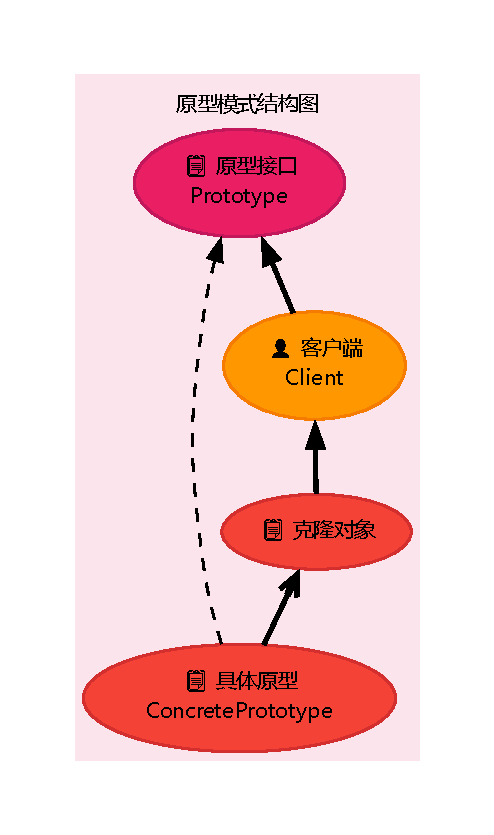
\includegraphics[width=0.9\textwidth]{images/prototype_pattern.pdf}
        \end{column}
        \begin{column}{0.58\textwidth}
            \begin{ytublock}{结构}
                \begin{itemize}
                    \item \textbf{原型接口(Prototype)}:定义克隆自身的抽象接口,通常包含 \texttt{clone()} 方法。
                    \item \textbf{具体原型(ConcretePrototype)}:实现原型接口,完成对象自身的深拷贝或浅拷贝。
                    \item \textbf{客户端(Client)}:通过调用原型的 \texttt{clone()} 方法,复制已有对象并生成新实例,而无需依赖具体类。
                    \item \textbf{克隆对象(ConcretePrototype2)}:克隆出来的对象。
                \end{itemize}
            \end{ytublock}
        \end{column}
    \end{columns}
\end{frame}

\begin{frame}{原型模式举例说明}
    \begin{exampleytublock}{游戏系统——道具批量生成}
        假设我们要开发一个游戏系统,需要批量生成不同类型的道具(如武器、防具、药水),每种道具有不同的属性(如攻击力、防御力、恢复量)和特殊效果(如中毒、加速、回血)。这些道具结构复杂,初始化参数繁多,手动创建既繁琐又容易出错。
        \textbf{原型模式}的实现思路如下:
        \begin{itemize}
            \item 定义道具产品的抽象类(如\texttt{Item}),所有具体道具类(如\texttt{武器}、\texttt{防具}、\texttt{药水})都继承自它。
            \item 定义道具属性的抽象类(如\texttt{ItemAttribute}),所有具体属性类(如\texttt{攻击力}、\texttt{防御力}、\texttt{恢复量})都继承自它。
            \item 定义道具效果的抽象类(如\texttt{ItemEffect}),所有具体效果类(如\texttt{中毒}、\texttt{加速}、\texttt{回血})都继承自它。
            \item 在\texttt{Item}类中声明\texttt{clone()}方法,作为原型接口。
            \item 各具体道具类实现\texttt{clone()}方法,实现自身的深拷贝或浅拷贝。
            \item 先创建一个标准的道具对象作为原型,后续通过调用其\texttt{clone()}方法,快速生成大量相似但内容不同的新道具对象,并根据需要调整属性或效果。
        \end{itemize}
    \end{exampleytublock}
\end{frame}

\begin{frame}{原型模式示例(道具属性)}
    \begin{columns}
        \begin{column}{0.48\textwidth}
            \inputminted[firstline=1, lastline=17]{cpp}{code/prototype_pattern.cpp}
        \end{column}
        \begin{column}{0.48\textwidth}
            \inputminted[firstline=19, lastline=30]{cpp}{code/prototype_pattern.cpp}
        \end{column}
    \end{columns}
\end{frame}

\begin{frame}{原型模式示例(道具属性)}
    \begin{columns}
        \begin{column}{0.48\textwidth}
            \inputminted[firstline=32, lastline=43]{cpp}{code/prototype_pattern.cpp}
        \end{column}
        \begin{column}{0.48\textwidth}
            \inputminted[firstline=45, lastline=56]{cpp}{code/prototype_pattern.cpp}
        \end{column}
    \end{columns}
\end{frame}

\begin{frame}{原型模式示例(道具效果)}
    \begin{columns}
        \begin{column}{0.48\textwidth}
            \inputminted[firstline=58, lastline=75]{cpp}{code/prototype_pattern.cpp}
        \end{column}
        \begin{column}{0.48\textwidth}
            \inputminted[firstline=77, lastline=97]{cpp}{code/prototype_pattern.cpp}
        \end{column}
    \end{columns}
\end{frame}

\begin{frame}{原型模式示例(道具)}
    \begin{columns}
        \begin{column}{0.48\textwidth}
            \inputminted[firstline=99, lastline=118]{cpp}{code/prototype_pattern.cpp}
        \end{column}
        \begin{column}{0.48\textwidth}
            \inputminted[firstline=119, lastline=136]{cpp}{code/prototype_pattern.cpp}
        \end{column}
    \end{columns}
\end{frame}

\begin{frame}{原型模式示例(道具)}
    \begin{columns}
        \begin{column}{0.48\textwidth}
            \inputminted[firstline=138, lastline=150]{cpp}{code/prototype_pattern.cpp}
        \end{column}
        \begin{column}{0.48\textwidth}
            \inputminted[firstline=151, lastline=167]{cpp}{code/prototype_pattern.cpp}
        \end{column}
    \end{columns}
\end{frame}

\begin{frame}{原型模式示例(道具)}
    \begin{columns}
        \begin{column}{0.48\textwidth}
            \inputminted[firstline=167, lastline=181]{cpp}{code/prototype_pattern.cpp}
        \end{column}
        \begin{column}{0.48\textwidth}
            \inputminted[firstline=182, lastline=198]{cpp}{code/prototype_pattern.cpp}
        \end{column}
    \end{columns}
\end{frame}

\begin{frame}{原型模式示例(原型管理)}
    \begin{columns}
        \begin{column}{0.48\textwidth}
            \inputminted[firstline=200, lastline=212]{cpp}{code/prototype_pattern.cpp}
        \end{column}
        \begin{column}{0.48\textwidth}
            \inputminted[firstline=220, lastline=237]{cpp}{code/prototype_pattern.cpp}
        \end{column}
    \end{columns}
\end{frame}

\begin{frame}{原型模式示例(原型使用)}
    \begin{columns}
        \begin{column}{0.48\textwidth}
            \inputminted[firstline=239, lastline=254]{cpp}{code/prototype_pattern.cpp}
        \end{column}
        \begin{column}{0.48\textwidth}
            \inputminted[firstline=256, lastline=270]{cpp}{code/prototype_pattern.cpp}
        \end{column}
    \end{columns}
\end{frame}

\begin{frame}{原型模式优缺点}
    \begin{ytublock}{优点}
        \begin{itemize}
            \item 可以在运行时动态创建对象,避免类创建时的复杂依赖。
            \item 创建新对象的效率高,适合需要大量相似对象的场景。
            \item 简化对象的创建过程,减少子类的数量。
            \item 可以方便地扩展和修改原型对象,灵活性高。
        \end{itemize}
    \end{ytublock}
    \begin{alertytublock}{缺点}
        \begin{itemize}
            \item 需要实现复杂对象的深拷贝,可能增加开发难度。
            \item 每个类都要配备克隆方法,代码维护成本较高。
            \item 对包含循环引用或复杂资源的对象克隆时容易出错。
        \end{itemize}
    \end{alertytublock}
\end{frame}

\section{结构型模式}
\begin{frame}{目录}
    \begin{multicols}{2}
        \tableofcontents[currentsection,hideothersubsections]
    \end{multicols}
\end{frame}

\begin{frame}{结构型模式(Structural Patterns)}
    \begin{ytublock}{什么是结构型模式}
        结构型模式关注的是"如何将类和对象进行组合",以构建更大、更灵活的系统结构。
        它们通过合理地组织类和对象之间的关系,使系统更易于扩展和维护。
        结构型模式强调"组合优于继承",通过组合已有的类和对象来获得新的功能,而不是单纯依赖继承。

        这些模式可以帮助我们简化系统结构、优化类之间的协作、提高代码复用性,并且让系统更容易适应变化。

        常见的结构型模式有:
        适配器模式(接口转换)、
        桥接模式(抽象分离)、
        组合模式(树形结构)、
        装饰器模式(动态扩展)、
        外观模式(简化接口)、
        享元模式(对象共享)、
        代理模式(访问控制)等。

        每种模式都有其独特的应用场景,比如需要兼容不同接口、动态添加功能、
        统一子系统入口、节省内存、控制访问等,都可以用结构型模式来解决。
    \end{ytublock}
\end{frame}

\begin{frame}{结构型模式}
    \begin{ytublock}{结构型模式简介}
        结构型模式(Structural Patterns)主要关注如何将类和对象进行组合,从而形成更大、更灵活的结构。它们通过合理地组织类和对象之间的关系,使系统更易于扩展和维护。结构型模式的核心思想是"组合优于继承",强调通过组合已有的类和对象来获得新的功能,而不是通过继承来扩展行为。
        {\small
        \begin{itemize}
            \item \textbf{适配器模式(Adapter Pattern)}:将一个类的接口转换成客户期望的另一个接口,使原本由于接口不兼容而不能一起工作的类可以协同工作。
            \item \textbf{桥接模式(Bridge Pattern)}:将抽象部分与实现部分分离,使它们可以独立变化,适用于系统需要在多个维度上扩展时。
            \item \textbf{组合模式(Composite Pattern)}:将对象组合成树形结构以表示"部分-整体"的层次结构,使客户端对单个对象和组合对象的使用具有一致性。
            \item \textbf{装饰器模式(Decorator Pattern)}:动态地给对象添加一些额外的职责,就增加功能来说,装饰器模式比生成子类更为灵活。
            \item \textbf{外观模式(Facade Pattern)}:为子系统中的一组接口提供一个统一的高层接口,使子系统更易使用。
            \item \textbf{享元模式(Flyweight Pattern)}:运用共享技术有效地支持大量细粒度对象的复用,节省内存。
            \item \textbf{代理模式(Proxy Pattern)}:为其他对象提供一种代理以控制对这个对象的访问,可以在访问对象时引入额外的操作(如权限控制、延迟加载等)。
        \end{itemize}
        }
    \end{ytublock}
\end{frame}

\subsection{适配器模式(Adapter Pattern)}

\begin{frame}{适配器模式(Adapter Pattern)}
    \textbf{适配器模式(Adapter Pattern)}是一种重要的结构型设计模式。
    它的核心思想是:\textbf{将一个类的接口转换成客户期望的另一个接口},使原本由于接口不兼容而不能一起工作的类可以协同工作。
    适配器模式通常用于系统集成、第三方库适配、老系统升级等场景,极大地提升了系统的灵活性和可扩展性。

    \begin{ytublock}{适用场景}
        \begin{itemize}
            \item 希望复用某个现有类,但其接口与当前系统不兼容。
            \item 需要创建一个可复用的类,使其能与其他接口各异的类协同工作。
            \item 不希望修改已有代码的前提下,适配第三方库或遗留系统。
            \item 系统需要使用一些现有的类,但这些类的接口不符合你的需求。
            \item 希望通过引入适配器,统一多个类的接口,简化客户端调用。
        \end{itemize}
    \end{ytublock}
\end{frame}

\begin{frame}{适配器模式结构}
    \begin{columns}
        \begin{column}{0.38\textwidth}
            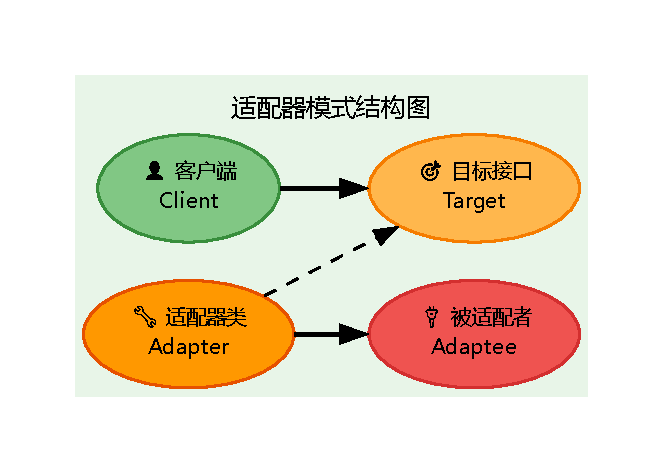
\includegraphics[width=1.0\textwidth]{images/adapter_pattern.pdf}
        \end{column}
        \begin{column}{0.58\textwidth}
            \begin{ytublock}{结构}
                \begin{itemize}
                    \item \textbf{目标接口(Target)}:客户端所期望的接口。
                    \item \textbf{被适配者(Adaptee)}:现有的、需要适配的类,其接口与目标接口不兼容。
                    \item \textbf{适配器(Adapter)}:通过包装一个被适配者对象,将其接口转换为目标接口,使其能够被客户端使用。
                \end{itemize}
            \end{ytublock}
        \end{column}
    \end{columns}
\end{frame}

\begin{frame}{适配器模式举例说明}
    \begin{exampleytublock}{音频播放器系统——适配器模式}
        假设我们有一个音频播放器系统,原本只支持播放MP3格式的音频文件(\texttt{Mp3Player}),现在需要支持播放MP4和VLC格式的文件,但不希望修改原有的播放器代码。此时可以通过适配器模式来实现兼容。
        \textbf{适配器模式}的实现思路如下:
        \begin{itemize}
            \item 定义一个目标接口(如\texttt{MediaPlayer}),声明统一的播放方法(如\texttt{play(fileType, fileName)})。
            \item 已有的\texttt{Mp3Player}类实现\texttt{MediaPlayer}接口,只能播放MP3文件。
            \item 新增\texttt{AdvancedMediaPlayer}接口,声明\texttt{playMp4()}和\texttt{playVlc()}等高级播放方法。
            \item 分别实现\texttt{AdvancedMediaPlayer}接口的\texttt{Mp4Player}和\texttt{VlcPlayer}类,分别支持MP4和VLC格式。
            \item 创建\texttt{MediaAdapter}适配器类,实现\texttt{MediaPlayer}接口,内部组合\texttt{AdvancedMediaPlayer},根据文件类型委托给对应的高级播放器。
            \item 客户端只依赖\texttt{MediaPlayer}接口,通过\texttt{MediaAdapter}即可无缝播放多种格式的音频文件,无需修改原有播放器代码。
        \end{itemize}
    \end{exampleytublock}
\end{frame}

\begin{frame}{适配器模式示例(目标接口)}
    \begin{columns}
        \begin{column}{0.48\textwidth}
            \inputminted[firstline=7, lastline=24]{cpp}{code/adapter_pattern.cpp}
        \end{column}
        \begin{column}{0.48\textwidth}
            \inputminted[firstline=25, lastline=42]{cpp}{code/adapter_pattern.cpp}
        \end{column}
    \end{columns}
\end{frame}

\begin{frame}{适配器模式示例(适配器)}
    \begin{columns}
        \begin{column}{0.48\textwidth}
            \inputminted[firstline=44, lastline=61]{cpp}{code/adapter_pattern.cpp}
        \end{column}
        \begin{column}{0.48\textwidth}
            \inputminted[firstline=62, lastline=75]{cpp}{code/adapter_pattern.cpp}
        \end{column}
    \end{columns}
\end{frame}

\begin{frame}{适配器模式示例(客户端)}
    \begin{columns}
        \begin{column}{0.48\textwidth}
            \inputminted[firstline=77, lastline=96]{cpp}{code/adapter_pattern.cpp}
        \end{column}
        \begin{column}{0.48\textwidth}
            \inputminted[firstline=98, lastline=118]{cpp}{code/adapter_pattern.cpp}
        \end{column}
    \end{columns}
\end{frame}

\begin{frame}{适配器模式优缺点}
    \begin{ytublock}{优点}
        \begin{itemize}
            \item 提高了类的复用性和系统的灵活性,无需修改原有代码即可兼容新接口。
            \item 遵循开闭原则,能够在不改变已有代码的基础上扩展系统功能。
            \item 客户端代码与具体实现解耦,便于后续维护和升级。
        \end{itemize}
    \end{ytublock}
    \begin{alertytublock}{缺点}
        \begin{itemize}
            \item 增加了系统的复杂度,过多使用适配器会导致系统结构混乱,难以维护。
            \item 适配器编写不当可能导致性能损耗或隐藏系统设计缺陷。
        \end{itemize}
    \end{alertytublock}
\end{frame}

\subsection{桥接模式(Bridge Pattern)}

\begin{frame}{桥接模式(Bridge Pattern)}
    桥接模式(Bridge Pattern)是一种结构型设计模式,它将抽象部分与其实现部分分离,使它们可以独立变化。
    桥接模式通过组合的方式将抽象与实现解耦,避免了继承带来的类爆炸问题,提高了系统的可扩展性和灵活性。
    \begin{ytublock}{适用场景}
        \begin{itemize}
            \item 希望抽象和实现可以独立扩展,且系统不希望两者之间有固定的绑定关系。
            \item 抽象和实现都有可能通过子类化进行扩展,并希望通过组合而非继承来实现它们之间的关联。
            \item 需要对抽象的实现部分进行修改时,不影响客户端代码。
            \item 希望在多个对象间共享实现,但又不希望客户知道实现的细节。
        \end{itemize}
    \end{ytublock}
\end{frame}

\begin{frame}{桥接模式结构}
    \begin{columns}
        \begin{column}{0.48\textwidth}
        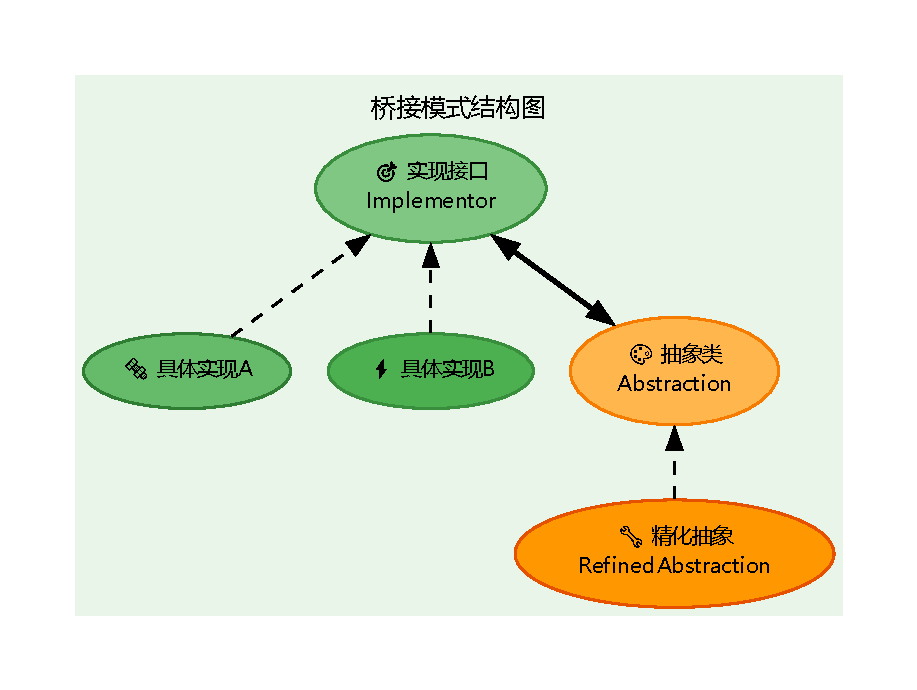
\includegraphics[width=1.0\textwidth]{images/bridge_pattern.pdf}
        \end{column}
        \begin{column}{0.48\textwidth}
            \begin{ytublock}{结构}
                \begin{itemize}
                    \item \textbf{抽象类(Abstraction)}:定义抽象接口,包含对实现部分的引用。
                    \item \textbf{实现接口(Implementor)}:定义实现接口,包含具体操作的实现。
                    \item \textbf{具体实现(Concrete Implementor)}:实现实现接口,提供具体操作的实现。
                    \item \textbf{精化抽象(Refined Abstraction)}:扩展抽象类,提供更具体的操作。
                \end{itemize}
            \end{ytublock}
        \end{column}
    \end{columns}
\end{frame}

\begin{frame}{桥接模式举例说明}
    \begin{exampleytublock}{音频播放器系统——桥接模式}
        假设我们有一个音频播放器系统,支持多种操作系统(如Windows、Linux、Mac),每种操作系统下都可以播放不同格式的音频文件(如MP3、MP4、VLC)。如果直接用继承方式实现,每增加一种操作系统或音频格式都需要大量子类,系统会变得非常复杂。此时可以通过\textbf{桥接模式}来解耦"操作系统平台"与"音频格式"的变化。
        \textbf{桥接模式}的实现思路如下:
        \begin{itemize}
            \item 定义\texttt{AudioFormat}实现接口,声明如\texttt{play(const std::string\& fileName)}等方法,具体实现如\texttt{Mp3Format}、\texttt{Mp4Format}、\texttt{VlcFormat}分别实现不同格式的播放。
            \item 定义\texttt{Player}抽象类,内部持有\texttt{AudioFormat}接口的指针或引用,声明如\texttt{play(const std::string\& fileName)}等方法。
            \item 具体的\texttt{Player}子类如\texttt{WindowsPlayer}、\texttt{LinuxPlayer}、\texttt{MacPlayer},在\texttt{play}方法中调用\texttt{AudioFormat}的实现,实现平台与格式的解耦。
            \item 客户端可以灵活组合不同的\texttt{Player}和\texttt{AudioFormat},如"Windows+MP3"、"Linux+MP4"等,无需为每种组合创建新子类。
        \end{itemize}
    \end{exampleytublock}
\end{frame}

\begin{frame}{桥接模式示例(实现接口)}
    \begin{columns}
        \begin{column}{0.48\textwidth}
            \inputminted[firstline=1, lastline=20]{cpp}{code/bridge_pattern.cpp}
        \end{column}
        \begin{column}{0.48\textwidth}
            \inputminted[firstline=21, lastline=37]{cpp}{code/bridge_pattern.cpp}
        \end{column}
    \end{columns}
\end{frame}

\begin{frame}{桥接模式示例(抽象类)}
    \begin{columns}
        \begin{column}{0.48\textwidth}
            \inputminted[firstline=39, lastline=57]{cpp}{code/bridge_pattern.cpp}
        \end{column}
        \begin{column}{0.48\textwidth}
            \inputminted[firstline=59, lastline=77]{cpp}{code/bridge_pattern.cpp}
        \end{column}
    \end{columns}
\end{frame}

\begin{frame}{桥接模式示例(客户端)}
    \begin{columns}
        \begin{column}{0.48\textwidth}
            \inputminted[firstline=79, lastline=92]{cpp}{code/bridge_pattern.cpp}
        \end{column}
        \begin{column}{0.48\textwidth}
            \inputminted[firstline=94, lastline=104]{cpp}{code/bridge_pattern.cpp}
        \end{column}
    \end{columns}
\end{frame}

\begin{frame}{桥接模式优缺点}
    \begin{ytublock}{优点}
        \begin{itemize}
            \item 分离抽象与实现,使它们可以独立变化,降低耦合度。
            \item 扩展性好,新增抽象或实现部分都很方便,无需修改原有代码。
            \item 实现细节对客户透明,客户端只需关注抽象接口。
            \item 有助于系统分层。
            \item 可以动态组合不同的实现,灵活应对多维度变化。
        \end{itemize}
    \end{ytublock}
    \begin{alertytublock}{缺点}
        \begin{itemize}
            \item 增加系统设计的复杂度,理解和实现成本较高。
            \item 桥接模式引入了更多的抽象层,可能导致代码结构变得更加抽象。
            \item 对于简单场景,使用桥接模式可能会导致"杀鸡用牛刀"。
        \end{itemize}
    \end{alertytublock}
\end{frame}

\subsection{组合模式(Composite Pattern)}

\begin{frame}{组合模式(Composite Pattern)}
    组合模式是一种结构型设计模式,它将对象组织成树形结构以表示"部分-整体"的层次关系。
    组合模式使得用户对单个对象和组合对象的使用具有一致性,无需关心它们的具体类型。
    \begin{ytublock}{适用场景}
        \begin{itemize}
            \item 需要表示对象的部分-整体层次结构,如树形菜单、文件系统等。
            \item 希望用户可以统一地处理单个对象和组合对象,无需区分它们。
        \end{itemize}
    \end{ytublock}
\end{frame}

\begin{frame}{组合模式结构}
    \begin{ytublock}{结构}
        \begin{itemize}
            \item \textbf{组件接口(Component)}:定义组合对象和叶子对象的公共接口。
            \item \textbf{叶子节点(Leaf)}:表示组合中的叶节点,不包含子组件。
            \item \textbf{组合节点(Composite)}:表示组合中的非叶节点,包含子组件。
        \end{itemize}
    \end{ytublock}
    \begin{center}
        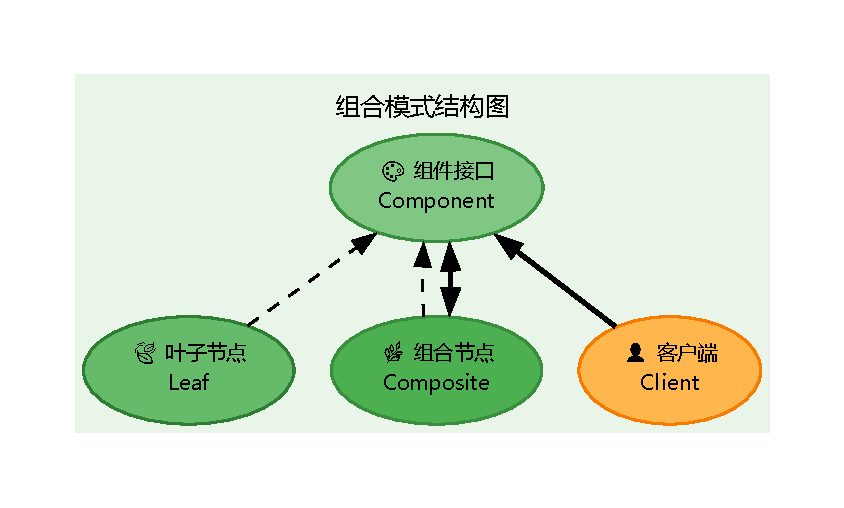
\includegraphics[width=0.65\textwidth]{images/composite_pattern.pdf}
    \end{center}
\end{frame}

\begin{frame}{组合模式举例说明}
    \begin{exampleytublock}{文件系统——树形结构}
        假设我们要实现一个文件系统,文件系统中有文件和文件夹两种类型。
        文件夹可以包含子文件夹和文件,形成树形的层级结构。
        我们可以使用组合模式来表示这种文件系统结构。
        \textbf{组合模式}的实现思路如下:
        \begin{itemize}
            \item 定义\texttt{Component}组件接口,包含如\texttt{add(Component)}、\texttt{remove(Component)}等方法。
            \item 定义\texttt{Leaf}叶子节点类,实现\texttt{Component}接口,表示文件。
            \item 定义\texttt{Composite}组合节点类,实现\texttt{Component}接口,表示文件夹。
        \end{itemize}
    \end{exampleytublock}
\end{frame}

\begin{frame}{组合模式示例(组件)}
    \begin{columns}
        \begin{column}{0.48\textwidth}
            \inputminted[firstline=1, lastline=18]{cpp}{code/composite_pattern.cpp}
        \end{column}
        \begin{column}{0.48\textwidth}
            \inputminted[firstline=19, lastline=36]{cpp}{code/composite_pattern.cpp}
        \end{column}
    \end{columns}
\end{frame}

\begin{frame}{组合模式示例(组件使用)}
    \begin{columns}
        \begin{column}{0.48\textwidth}
            \inputminted[firstline=42, lastline=54]{cpp}{code/composite_pattern.cpp}
        \end{column}
        \begin{column}{0.48\textwidth}
            \inputminted[firstline=55, lastline=66]{cpp}{code/composite_pattern.cpp}
        \end{column}
    \end{columns}
\end{frame}

\begin{frame}{组合模式优缺点}
    \begin{ytublock}{优点}
        \begin{itemize}
            \item 简化客户端代码,统一处理单个对象和组合对象。
            \item 简化系统结构,使得系统更易于扩展。
            \item 提高代码复用性,组合对象可以重用。
        \end{itemize}
    \end{ytublock}
    \begin{alertytublock}{缺点}
        \begin{itemize}
            \item 可能会导致系统设计变得复杂,难以理解。
            \item 组合模式可能会导致系统性能下降,因为需要遍历整个组合树。
        \end{itemize}
    \end{alertytublock}
\end{frame}

\subsection{装饰器模式(Decorator Pattern)}

\begin{frame}{装饰器模式(Decorator Pattern)}
    \textbf{装饰器模式}是一种结构型设计模式,允许在不修改原有对象结构的情况下,动态地为对象添加额外的功能。
    与通过继承生成子类相比,装饰器模式更加灵活,能够实现功能的按需组合和扩展
    \textbf{核心思想}使用一系列装饰器类将原始对象"包裹"起来,每个装饰器都可以在保持原有接口的前提下,增加新的行为或责任。

    \begin{ytublock}{适用场景}
        \begin{itemize}
            \item 需要在运行时为对象动态添加功能,且这些功能可以灵活组合。
            \item 希望通过组合而非继承的方式扩展对象的行为,避免类爆炸。
            \item 希望对核心类的功能进行增强,但又不希望影响到其他对象。
            \item 需要实现可撤销的职责或临时性的功能增强。
        \end{itemize}
    \end{ytublock}
\end{frame}

\begin{frame}{装饰器模式结构}
    \begin{columns}
        \begin{column}{0.48\textwidth}
            \begin{ytublock}{结构}
                \begin{itemize}
                    \item \textbf{组件接口(Component)}:定义组件的公共接口。
                    \item \textbf{具体组件(Concrete Component)}:表示具体的组件类,实现组件接口。
                    \item \textbf{装饰器(Decorator)}:表示装饰器类,包含对组件的引用,实现组件接口。
                    \item \textbf{具体装饰器(Concrete Decorator)}:表示具体的装饰器类,实现装饰器接口。
                \end{itemize}
            \end{ytublock}
        \end{column}
        \begin{column}{0.48\textwidth}
            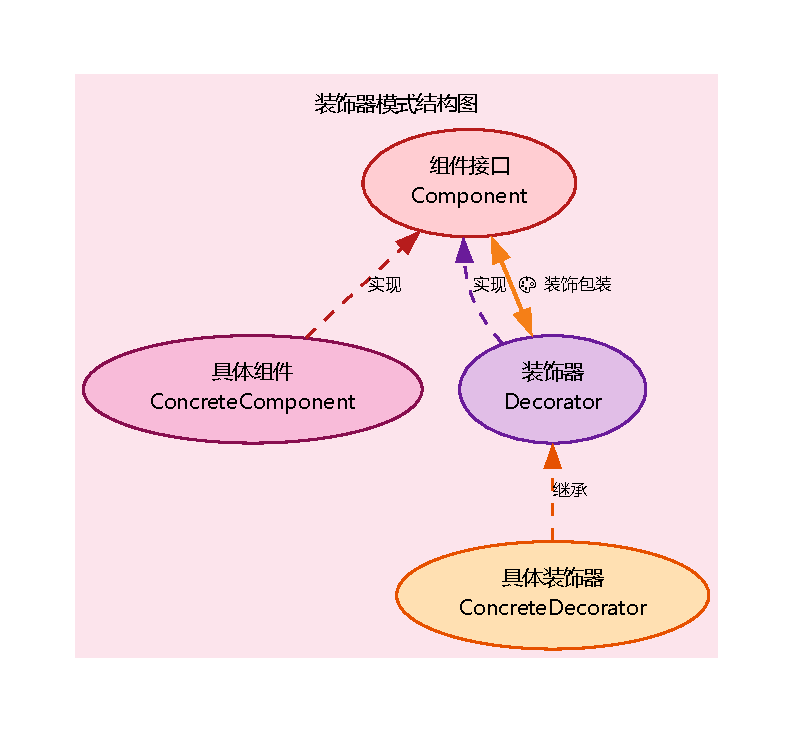
\includegraphics[width=1.0\textwidth]{images/decorator_pattern.pdf}
        \end{column}
    \end{columns}
\end{frame}

\begin{frame}{装饰器模式举例说明}
    \begin{exampleytublock}{音乐播放器——动态扩展功能}
        假设我们有一个音乐播放器,播放器本身可以播放音频文件。
        现在我们希望在不修改播放器核心代码的情况下,动态地为播放器增加新的功能,比如"均衡器"、"音量增强"、"歌词显示"等。
        此时可以使用装饰器模式来实现功能的灵活扩展。
        \textbf{装饰器模式}的实现思路如下:
        \begin{itemize}
            \item 定义\texttt{Player}组件接口,包含如\texttt{play()}等方法。
            \item 定义\texttt{ConcretePlayer}具体组件类,实现\texttt{Player}接口,负责基础的播放功能。
            \item 定义\texttt{PlayerDecorator}装饰器类,持有\texttt{Player}接口的引用,并实现\texttt{Player}接口。
            \item 定义\texttt{ConcreteDecorator}具体装饰器类,实现\texttt{PlayerDecorator},如"均衡器"、"音量增强"等,扩展播放器功能。
        \end{itemize}
    \end{exampleytublock}
\end{frame}

\begin{frame}{装饰器模式示例(客户端+装饰器)}
    \begin{columns}
        \begin{column}{0.48\textwidth}
            \inputminted[firstline=1, lastline=18]{cpp}{code/decorator_pattern.cpp}
        \end{column}
        \begin{column}{0.48\textwidth}
            \inputminted[firstline=20, lastline=36]{cpp}{code/decorator_pattern.cpp}
        \end{column}
    \end{columns}
\end{frame}

\begin{frame}{装饰器模式示例(装饰器使用)}
    \begin{columns}
        \begin{column}{0.48\textwidth}
            \inputminted[firstline=38, lastline=55]{cpp}{code/decorator_pattern.cpp}
        \end{column}
        \begin{column}{0.48\textwidth}
            \inputminted[firstline=67, lastline=77]{cpp}{code/decorator_pattern.cpp}
        \end{column}
    \end{columns}
\end{frame}

\begin{frame}{装饰器模式优缺点}
    \begin{ytublock}{优点}
        \begin{itemize}
            \item 灵活性高,可以在运行时动态地为对象添加功能。
            \item 可以组合多个装饰器,实现复杂的功能。
            \item 可以实现可撤销的职责。
        \end{itemize}
    \end{ytublock}
    \begin{alertytublock}{缺点}
        \begin{itemize}
            \item 可能会导致系统设计变得复杂,难以理解。
            \item 装饰器模式可能会导致系统性能下降,因为需要遍历整个装饰器链。
        \end{itemize}
    \end{alertytublock}
\end{frame}

\subsection{外观模式(Facade Pattern)}

\begin{frame}{外观模式(Facade Pattern)}
    外观模式是一种结构型设计模式,通过为子系统中的一组接口提供一个统一的高层接口,使得子系统更加易用。
    它将复杂子系统的内部实现细节对外部屏蔽,客户端只需与外观对象交互即可完成复杂操作,从而降低了系统的耦合度。

    \begin{ytublock}{适用场景}
        \begin{itemize}
            \item 希望为复杂子系统提供一个简单统一的入口。
            \item 客户端与多个子系统存在较强依赖,希望通过外观模式降低耦合。
            \item 需要分层设计时,可以使用外观模式作为每一层的入口,简化层与层之间的交互。
        \end{itemize}
    \end{ytublock}
\end{frame}

\begin{frame}{外观模式结构}
    \begin{columns}
        \begin{column}{0.48\textwidth}
            \begin{ytublock}{结构}
                \begin{itemize}
                    \item \textbf{外观(Facade)}:提供简单接口,封装子系统复杂操作。
                    \item \textbf{子系统(Subsystem)}:实现具体业务逻辑,被外观类调用。
                \end{itemize}
            \end{ytublock}
        \end{column}
        \begin{column}{0.48\textwidth}
            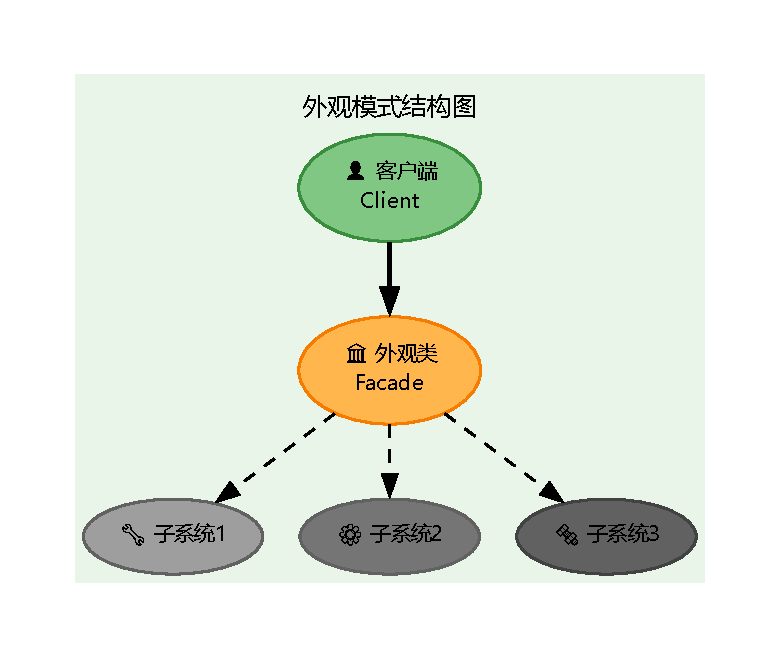
\includegraphics[width=1.0\textwidth]{images/facade_pattern.pdf}
        \end{column}
    \end{columns}
\end{frame}

\begin{frame}{外观模式举例说明}
    \begin{exampleytublock}{智能家居系统——回家模式}
        假设我们有一个智能家居系统,系统本身包含多个子系统:智能灯光、智能空调、安全监控等。
        现在我们希望用户只需按一个按钮即可完成"回家模式"这一系列操作,而无需分别操作每个子系统。
        此时可以使用外观模式来实现功能的简化和统一。
        \textbf{外观模式}的实现思路如下:
        \begin{itemize}
            \item 定义各个子系统的接口和实现类,如\texttt{LightSystem}、\texttt{AirConditioner}、\texttt{SecuritySystem}等,分别负责各自的功能。
            \item 定义\texttt{SmartHomeFacade}外观类,内部组合各个子系统对象,封装复杂的操作流程。
            \item 用户只需调用\texttt{SmartHomeFacade}的\texttt{enterHomeMode()}等简单方法,即可一键完成回家模式的所有操作,无需关心子系统的具体细节。
        \end{itemize}
    \end{exampleytublock}
\end{frame}

\begin{frame}{外观模式示例(子系统)}
    \begin{columns}
        \begin{column}{0.48\textwidth}
            \inputminted[firstline=1, lastline=15]{cpp}{code/facade_pattern.cpp}
        \end{column}
        \begin{column}{0.48\textwidth}
            \inputminted[firstline=17, lastline=32]{cpp}{code/facade_pattern.cpp}
        \end{column}
    \end{columns}
\end{frame}

\begin{frame}{外观模式示例(外观类)}
    \begin{columns}
        \begin{column}{0.48\textwidth}
            \inputminted[firstline=34, lastline=45]{cpp}{code/facade_pattern.cpp}
        \end{column}
        \begin{column}{0.48\textwidth}
            \inputminted[firstline=47, lastline=66]{cpp}{code/facade_pattern.cpp}
        \end{column}
    \end{columns}
\end{frame}

\begin{frame}{外观模式示例(客户端)}
    \inputminted[firstline=72, lastline=82]{cpp}{code/facade_pattern.cpp}
\end{frame}

\begin{frame}{外观模式优缺点}
    \begin{ytublock}{优点}
        \begin{itemize}
            \item 简化客户端使用,降低耦合度。
            \item 客户端只需与外观类交互。
            \item 增强系统可扩展性,易于维护和修改。
        \end{itemize}
    \end{ytublock}
    \begin{alertytublock}{缺点}
        \begin{itemize}
            \item 可能引入额外复杂度,如果外观类过于复杂。
            \item 对原有子系统改动较大。
        \end{itemize}
    \end{alertytublock}
\end{frame}

\subsection{享元模式(Flyweight Pattern)}

\begin{frame}{享元模式(Flyweight Pattern)}
    享元模式的核心思想是:\textbf{通过共享技术,减少内存中对象的数量},从而有效支持大量细粒度对象的高效复用。
    如果一个程序中有很多内容相似、重复的对象,我们可以把它们的"相同部分"提取出来共享,
    只为"不同部分"单独存储,这样可以大大节省内存。
    \begin{ytublock}{适用场景}
        \begin{itemize}
            \item 程序中需要大量相似对象,导致内存占用大。
            \item 对象的大部分状态可以提取出来作为共享(内部状态),只有少部分信息需要单独保存(外部状态)。
            \item 可以通过共享对象来替代大量重复对象。
            \item 对象的身份(唯一性)不重要。
        \end{itemize}
    \end{ytublock}
\end{frame}

\begin{frame}{享元模式结构}
    \begin{columns}
        \begin{column}{0.38\textwidth}
            \begin{ytublock}{结构}
                \begin{itemize}
                    \item \textbf{享元接口(Flyweight)}:共享对象,包含内部状态。
                    \item \textbf{具体享元(Concrete Flyweight)}:实现享元接口,存储内部状态。
                    \item \textbf{享元工厂(Flyweight Factory)}:管理享元对象,提供获取享元对象的方法。
                \end{itemize}
            \end{ytublock}
        \end{column}
        \begin{column}{0.58\textwidth}
            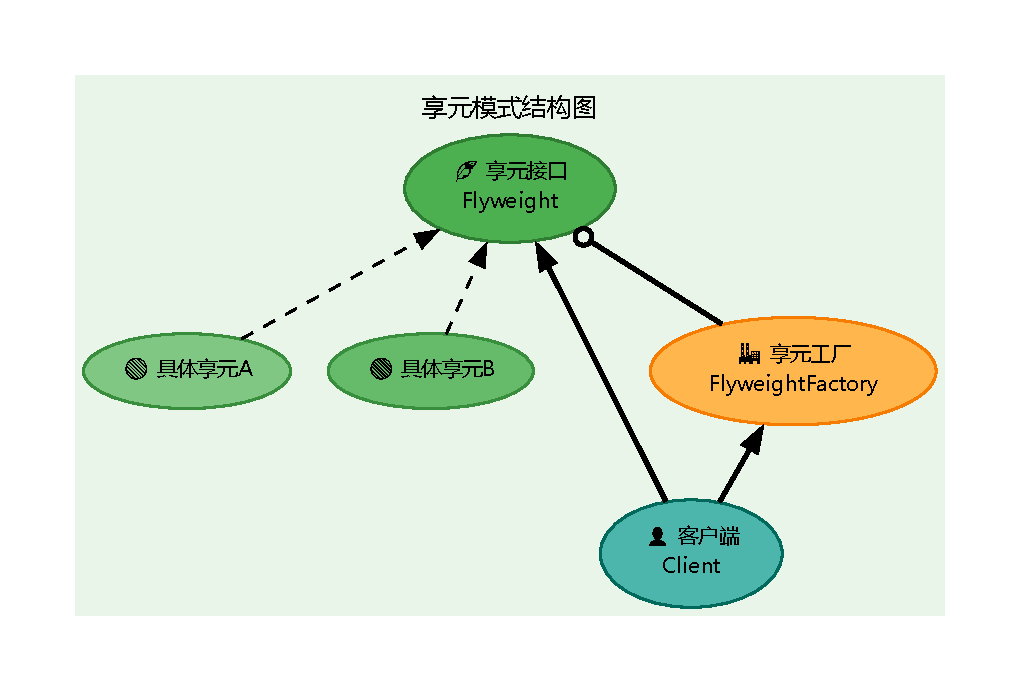
\includegraphics[width=1.0\textwidth]{images/flyweight_pattern.pdf}
        \end{column}
    \end{columns}
\end{frame}

\begin{frame}{享元模式举例说明}
    \begin{exampleytublock}{地图应用——树木图标共享}
        假设我们有一个地图应用,需要在地图上显示成千上万个树木图标。每棵树的种类有限,但位置和高度等信息各不相同。
        这时可以用享元模式来共享树的图标资源,只为每棵树单独保存位置等外部状态,从而大幅节省内存。
        \textbf{享元模式}的实现思路如下:
        \begin{itemize}
            \item 定义享元接口(\texttt{Tree}),包含树的图标等内部状态。
            \item 定义具体享元(\texttt{ConcreteTree}),实现享元接口,存储具体树种的图标等信息。
            \item 定义享元工厂(\texttt{TreeFactory}),管理和复用树种对象,提供获取享元对象的方法。
            \item 每棵树只保存位置、高度等外部状态,内部状态通过享元对象共享。
        \end{itemize}
    \end{exampleytublock}
\end{frame}

\begin{frame}{享元模式示例(享元接口与具体享元)}
    \begin{columns}
        \begin{column}{0.48\textwidth}
            \inputminted[firstline=1, lastline=15]{cpp}{code/flyweight_pattern.cpp}
        \end{column}
        \begin{column}{0.48\textwidth}
            \inputminted[firstline=17, lastline=28]{cpp}{code/flyweight_pattern.cpp}
        \end{column}
    \end{columns}
\end{frame}

\begin{frame}{享元模式示例(享元工厂)}
    \begin{columns}
        \begin{column}{0.48\textwidth}
            \inputminted[firstline=30, lastline=45]{cpp}{code/flyweight_pattern.cpp}
        \end{column}
        \begin{column}{0.48\textwidth}
            \inputminted[firstline=46, lastline=60]{cpp}{code/flyweight_pattern.cpp}
        \end{column}
    \end{columns}
\end{frame}

\begin{frame}{享元模式示例(客户端)}
    \begin{columns}
        \begin{column}{0.48\textwidth}
            \inputminted[firstline=62, lastline=77]{cpp}{code/flyweight_pattern.cpp}
        \end{column}
        \begin{column}{0.48\textwidth}
            \inputminted[firstline=78, lastline=86]{cpp}{code/flyweight_pattern.cpp}
        \end{column}
    \end{columns}
\end{frame}

\begin{frame}{享元模式示例(应用)}
    \inputminted[firstline=94, lastline=112]{cpp}{code/flyweight_pattern.cpp}
\end{frame}

\begin{frame}{享元模式优缺点}
    \begin{ytublock}{优点}
        \begin{itemize}
            \item 大量对象共享内部状态,极大节省内存。
            \item 外部状态独立存储,灵活管理。
            \item 适合地图、图标、粒子等场景。
        \end{itemize}
    \end{ytublock}
    \begin{alertytublock}{缺点}
        \begin{itemize}
            \item 需要将内部状态和外部状态分离,这可能会增加系统复杂度。
            \item 外部状态的管理可能比较繁琐。
        \end{itemize}
    \end{alertytublock}
\end{frame}

\subsection{代理模式(Proxy Pattern)}

\begin{frame}{代理模式(Proxy Pattern)}
    为其他对象提供一种代理,以控制对该对象的访问。
    代理对象在客户端和目标对象之间起到中介作用,可以在不改变目标对象的前提下,扩展或控制其访问方式。
    \begin{ytublock}{常见类型}
        \begin{itemize}
            \item \textbf{远程代理}:为位于不同地址空间的对象提供本地代表,实现远程通信。
            \item \textbf{虚拟代理}:根据需要创建开销较大的对象,实现延迟加载或按需创建。
            \item \textbf{保护代理}:控制对目标对象的访问权限,进行安全控制。
            \item \textbf{智能引用}:在访问对象时附加额外操作,如引用计数、日志记录等。
        \end{itemize}
    \end{ytublock}
    \begin{ytublock}{适用场景}
        \begin{itemize}
            \item 需要对目标对象的访问进行控制或增强时。
            \item 希望在不修改目标对象代码的情况下,增加额外功能(如缓存、安全、延迟加载等)。
            \item 需要为资源消耗大或敏感的对象提供统一的访问接口。
        \end{itemize}
    \end{ytublock}
\end{frame}

\begin{frame}{代理模式结构}
    \begin{ytublock}{结构组成}
        \begin{itemize}
            \item \textbf{Subject(抽象主题/接口)}:定义代理和真实对象的公共接口,确保两者可以互换。
            \item \textbf{RealSubject(真实主题)}:实现了Subject接口,提供实际的核心业务功能。
            \item \textbf{Proxy(代理类)}:同样实现Subject接口,内部持有RealSubject对象的引用,负责在客户端和真实对象之间进行控制和扩展(如权限校验、延迟加载、日志等)。
        \end{itemize}
    \end{ytublock}
    \begin{center}
        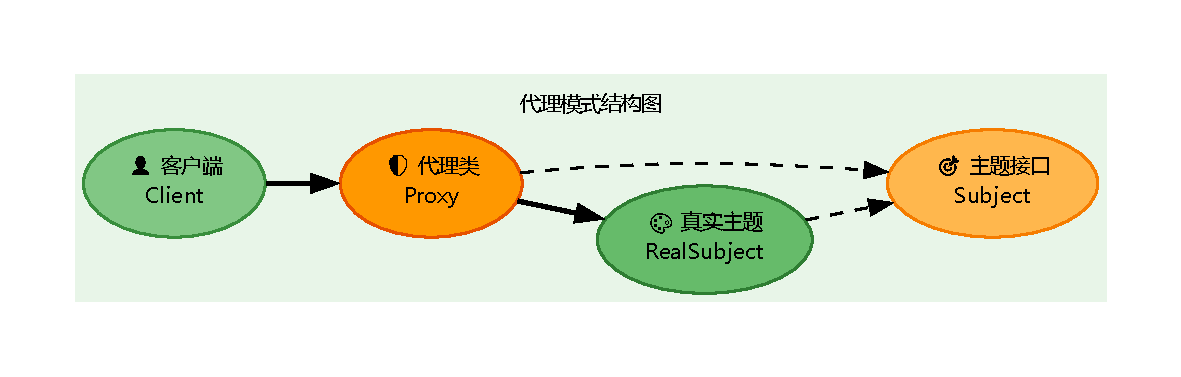
\includegraphics[width=0.99\textwidth]{images/proxy_pattern.pdf}
    \end{center}
\end{frame}

\begin{frame}{代理模式举例说明}
    \begin{exampleytublock}{虚拟代理:游戏资源的延迟加载}
        在大型游戏开发中,场景中通常包含大量高精度3D模型和贴图资源。这些资源文件体积庞大,加载耗时且占用大量内存。
        如果在游戏启动时一次性全部加载,容易导致启动缓慢、内存压力大。
        理想的做法是:\textbf{仅在玩家真正进入某个场景或靠近某个对象时,才加载对应资源}。
        此时,\textbf{虚拟代理}模式可以很好地解决这一问题。
        \textbf{实现思路如下:}
        \begin{itemize}
            \item 定义资源接口(\texttt{Subject}),如\texttt{load()}、\texttt{render()}等,统一资源的加载与显示操作。
            \item 实现真实资源类(\texttt{RealSubject}),负责真正从磁盘加载和渲染资源,构造时会读取大文件并初始化。
            \item 实现资源代理类(\texttt{Proxy}),同样实现资源接口,内部持有真实资源对象指针。只有在调用\texttt{load()}或\texttt{render()}时,才会真正创建和加载资源,实现延迟加载。
        \end{itemize}
    \end{exampleytublock}
\end{frame}

\begin{frame}{代理模式示例(主题类)}
    \begin{columns}
        \begin{column}{0.48\textwidth}
            \inputminted[firstline=1, lastline=14]{cpp}{code/proxy_pattern.cpp}
        \end{column}
        \begin{column}{0.48\textwidth}
            \inputminted[firstline=16, lastline=35]{cpp}{code/proxy_pattern.cpp}
        \end{column}
    \end{columns}
\end{frame}

\begin{frame}{代理模式示例(代理类)}
    \begin{columns}
        \begin{column}{0.48\textwidth}
            \inputminted[firstline=37, lastline=56]{cpp}{code/proxy_pattern.cpp}
        \end{column}
        \begin{column}{0.48\textwidth}
            \inputminted[firstline=64, lastline=82]{cpp}{code/proxy_pattern.cpp}
        \end{column}
    \end{columns}
\end{frame}

\begin{frame}{代理模式优缺点}
    \begin{ytublock}{优点}
        \begin{itemize}
            \item 控制对真实对象的访问,保护真实对象。
            \item 延迟对象的创建,提高性能。
            \item 统一接口,方便扩展。
        \end{itemize}
    \end{ytublock}
    \begin{alertytublock}{缺点}
        \begin{itemize}
            \item 增加了系统的复杂度。
            \item 代理对象和真实对象可能不一致,需要额外处理。
        \end{itemize}
    \end{alertytublock}
\end{frame}

\section{行为型模式}
\begin{frame}{目录}
    \begin{multicols}{2}
        \tableofcontents[currentsection,hideothersubsections]
    \end{multicols}
\end{frame}

\begin{frame}{行为型模式(Behavioral Patterns)}
    \begin{ytublock}{什么是行为型模式}
        行为型模式关注的是"对象之间如何协作与通信",即如何合理分配职责、组织对象之间的交互,从而实现更灵活、可扩展的系统行为。
        行为型模式不仅仅关注类和对象的结构,还强调它们之间的动态交互和职责划分。

        这些模式可以帮助我们降低对象之间的耦合度,优化职责分配,提高系统的灵活性和可维护性。

        常见的行为型模式有:
        责任链模式(请求传递)、
        命令模式(请求封装)、
        解释器模式(语言解析)、
        迭代器模式(顺序访问)、
        中介者模式(对象交互)、
        备忘录模式(状态保存)、
        观察者模式(事件通知)、
        状态模式(状态变迁)、
        策略模式(算法选择)、
        模板方法模式(算法框架)、
        访问者模式(双重分派)等。

        每种模式都有其独特的应用场景,比如请求链式处理、解耦发送者与接收者、动态切换算法、对象状态管理、事件通知等,都可以用行为型模式来解决。
    \end{ytublock}
\end{frame}

\begin{frame}{行为型模式}
    \begin{ytublock}{行为型模式概述(上)}
        行为型模式(Behavioral Patterns)关注对象之间的通信和职责分配,共有\textbf{11种经典模式}:
        \begin{itemize}
            \item \textbf{责任链模式}:将请求沿着处理链传递,避免请求发送者和接收者之间的耦合
            \item \textbf{命令模式}:将请求封装为对象,支持请求的排队、撤销和重做操作
            \item \textbf{解释器模式}:定义语言的文法表示,并定义一个解释器来解释语言中的句子
            \item \textbf{迭代器模式}:提供一种方法顺序访问一个聚合对象中各个元素,而又不暴露该对象的内部表示
            \item \textbf{中介者模式}:用一个中介对象来封装一系列的对象交互,使对象不需要显式地相互引用
            \item \textbf{备忘录模式}:在不破坏封装的前提下,捕获并保存一个对象的内部状态,以便稍后恢复
        \end{itemize}
    \end{ytublock}
\end{frame}

\begin{frame}{行为型模式}
    \begin{ytublock}{行为型模式概述(下)}
        \begin{itemize}
            \item \textbf{观察者模式}:定义对象间的一种一对多的依赖关系,当一个对象的状态发生改变时,所有依赖于它的对象都得到通知
            \item \textbf{状态模式}:允许一个对象在其内部状态改变时改变它的行为,对象看起来似乎修改了它的类
            \item \textbf{策略模式}:定义一系列的算法,把它们一个个封装起来,并且使它们可相互替换
            \item \textbf{模板方法模式}:定义一个操作中的算法的骨架,而将一些步骤延迟到子类中实现
            \item \textbf{访问者模式}:表示一个作用于某对象结构中的各元素的操作,使你可以在不改变各元素的类的前提下定义作用于这些元素的新操作
        \end{itemize}
    \end{ytublock}
\end{frame}

\subsection{责任链模式(Chain of Responsibility Pattern)}

\begin{frame}{责任链模式(Chain of Responsibility Pattern)}
    使多个对象都有机会处理请求,从而避免请求的发送者和接收者之间的耦合关系。
    将这些对象连成一条链,并沿着这条链传递该请求,直到有一个对象处理它为止。
    \begin{ytublock}{适用场景}
        \begin{itemize}
            \item 有多个对象可以处理一个请求,哪个对象处理该请求运行时刻自动确定。
            \item 想在不明确指定接收者的情况下,向多个对象中的一个提交一个请求。
            \item 可处理一个请求的对象集合应被动态指定。
        \end{itemize}
    \end{ytublock}
\end{frame}

\begin{frame}{责任链模式结构}
    \begin{columns}
        \begin{column}{0.48\textwidth}
            \begin{ytublock}{结构组成}
                \begin{itemize}
                    \item \textbf{Handler(抽象处理者)}:定义一个处理请求的接口,并实现后继链(successor)。
                    \item \textbf{ConcreteHandler(具体处理者)}:实现抽象处理者的处理方法,如果可以处理请求,则处理请求,否则将请求传递给后继者。
                    \item \textbf{Client(客户端)}:创建处理链,并向链的第一个处理者发送请求,开始处理过程。
                \end{itemize}
            \end{ytublock}
        \end{column}
        \begin{column}{0.48\textwidth}
            \begin{center}
                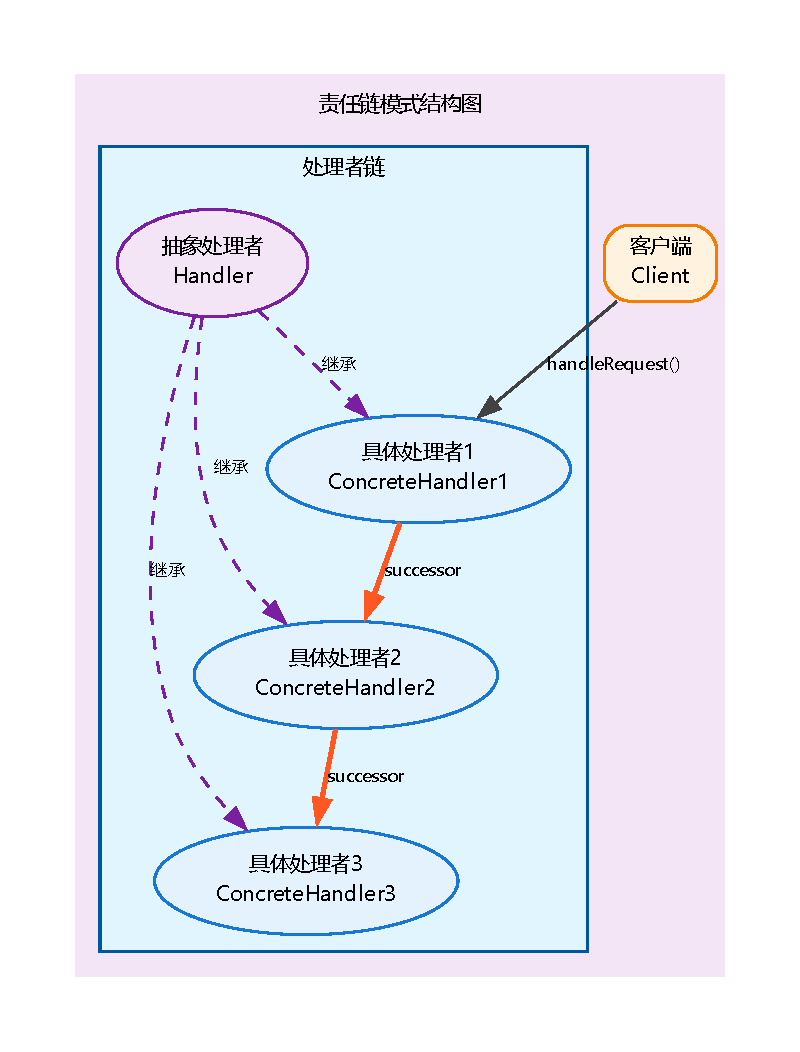
\includegraphics[width=0.8\textwidth]{images/chain_of_responsibility_pattern.pdf}
            \end{center}
        \end{column}
    \end{columns}
\end{frame}

\begin{frame}{责任链模式举例说明}
    \begin{exampleytublock}{技能效果责任链:多环节处理技能请求}
        在角色扮演类游戏中,角色释放技能时,技能的最终效果往往需要经过多个环节的处理。例如,技能伤害会先经过装备加成、再叠加Buff增益,最后还可能被护盾吸收。每个环节都可以对技能效果进行修改或拦截。理想的做法是:\textbf{将这些处理环节串联成一条责任链,技能请求依次传递,直到最终生效或被拦截}。
        \textbf{实现思路如下:}
        \begin{itemize}
            \item 定义技能处理接口(\texttt{Handler}),如\texttt{handleSkill()},并实现后继链(successor),统一技能请求的处理流程。
            \item 实现具体处理者类(\texttt{ConcreteHandler}),如装备处理器、Buff处理器、护盾处理器等,分别负责各自环节的处理逻辑。每个处理者判断是否处理当前请求,若不能处理则传递给下一个处理者。
            \item 客户端(\texttt{Client})负责创建技能处理链,并将技能请求交给链的起点,技能效果依次经过各个处理环节,最终得到处理结果。
        \end{itemize}
    \end{exampleytublock}
\end{frame}

\begin{frame}{责任链模式示例(抽象处理者)}
    \begin{columns}
        \begin{column}{0.48\textwidth}
            \inputminted[firstline=1, lastline=18]{cpp}{code/chain_of_responsibility_pattern.cpp}
        \end{column}
        \begin{column}{0.48\textwidth}
            \inputminted[firstline=20, lastline=36]{cpp}{code/chain_of_responsibility_pattern.cpp}
        \end{column}
    \end{columns}
\end{frame}

\begin{frame}{责任链模式示例(具体处理者)}
    \begin{columns}
        \begin{column}{0.48\textwidth}
            \inputminted[firstline=38, lastline=49]{cpp}{code/chain_of_responsibility_pattern.cpp}
        \end{column}
        \begin{column}{0.48\textwidth}
            \inputminted[firstline=51, lastline=62]{cpp}{code/chain_of_responsibility_pattern.cpp}
        \end{column}
    \end{columns}
\end{frame}

\begin{frame}{责任链模式示例(具体处理者)}
    \begin{columns}
        \begin{column}{0.48\textwidth}
            \inputminted[firstline=64, lastline=76]{cpp}{code/chain_of_responsibility_pattern.cpp}
        \end{column}
        \begin{column}{0.48\textwidth}
            \inputminted[firstline=78, lastline=87]{cpp}{code/chain_of_responsibility_pattern.cpp}
        \end{column}
    \end{columns}
\end{frame}

\begin{frame}{责任链模式示例(客户端)}
    \inputminted[firstline=96, lastline=115]{cpp}{code/chain_of_responsibility_pattern.cpp}
\end{frame}

\begin{frame}{责任链模式优缺点}
    \begin{ytublock}{优点}
        \begin{itemize}
            \item 降低对象之间的耦合度,使请求的发送者与接收者解耦,提高系统灵活性和可维护性。
            \item 支持动态地添加、删除或重组处理者,便于扩展和修改。
            \item 责任链可以灵活组合,支持多种处理顺序和策略,增强系统的可配置性。
            \item 每个处理者只需关注自身职责,便于代码复用。
        \end{itemize}
    \end{ytublock}
    \begin{alertytublock}{缺点}
        \begin{itemize}
            \item 可能导致请求在链上传递过长,影响性能,调试和排查较为困难。
            \item 责任链过长或不合理,可能导致某些请求得不到及时处理或丢失。
            \item 处理者之间的顺序依赖需要谨慎管理,否则可能出现逻辑错误。
        \end{itemize}
    \end{alertytublock}
\end{frame}

\subsection{解释器模式(Interpreter Pattern)}

\begin{frame}{解释器模式(Interpreter Pattern)}
    给定一种语言,定义其文法的一种表示,并定义一个解释器,利用该表示来解释语言中的句子。
    解释器模式常用于实现自定义脚本、表达式求值、规则引擎等场景。
    \begin{ytublock}{适用场景}
        \begin{itemize}
            \item 需要解释执行的语言,并且可以将语言中的句子表示为抽象语法树(AST)。
            \item 语言的文法结构相对简单,变化不频繁。
            \item 对执行效率要求不高,主要关注灵活性和可扩展性。
        \end{itemize}
    \end{ytublock}
\end{frame}

\begin{frame}{解释器模式结构}
    \begin{columns}
        \begin{column}{0.38\textwidth}
            \begin{ytublock}{结构组成}
                \begin{itemize}
                    \item \textbf{AbstractExpression(抽象表达式)}:定义解释器的接口,用于解释语法规则。
                    \item \textbf{TerminalExpression(终结符表达式)}:实现抽象表达式的解释方法,处理最基本的语法单元。
                    \item \textbf{NonTerminalExpression(非终结符表达式)}:实现抽象表达式的解释方法,处理复合语法单元。
                    \item \textbf{Context(上下文)}:包含解释器需要的数据,传递给抽象表达式。
                \end{itemize}
            \end{ytublock}
        \end{column}
        \begin{column}{0.58\textwidth}
            \begin{center}
                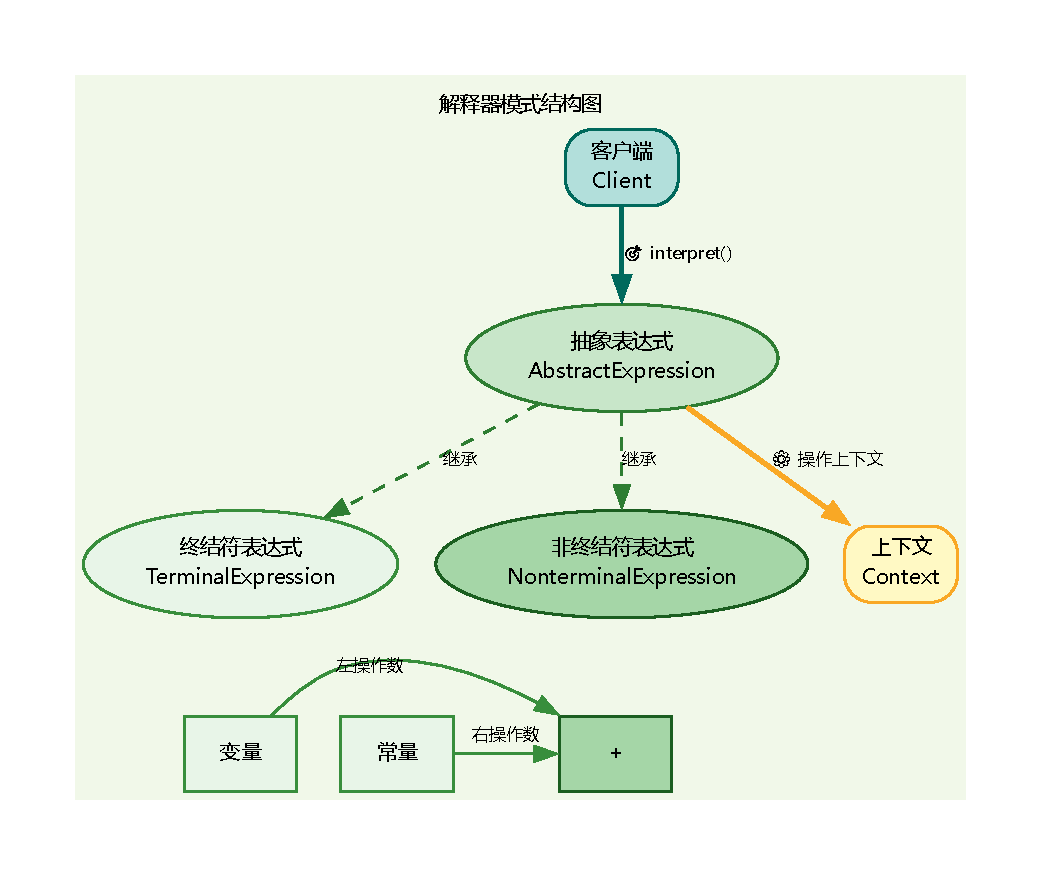
\includegraphics[width=1.0\textwidth]{images/interpreter_pattern.pdf}
            \end{center}
        \end{column}
    \end{columns}
\end{frame}

\begin{frame}{解释器模式举例说明}
    \begin{exampleytublock}{游戏中的解释器模式——属性公式解析}
        在一款角色扮演游戏中,角色的攻击力、伤害、暴击等属性往往需要根据策划配置的公式动态计算。例如"攻击力 = 力量 \texttt{*} 2 + 武器加成"。为了让策划可以灵活调整公式,系统需要支持表达式的解析与计算。此时可以采用解释器模式,将公式解析和计算过程解耦,结构如下:
        \begin{itemize}
            \item 定义抽象表达式(\texttt{AbstractExpression}),声明解释接口(如 \texttt{interpret(context)})。
            \item 实现终结符表达式(\texttt{TerminalExpression}),用于处理常量、变量(如"力量"、"武器加成"),直接返回对应值。
            \item 实现非终结符表达式(\texttt{NonTerminalExpression}),如加法、乘法等运算符,递归组合并解释子表达式。
            \item 定义上下文(\texttt{Context}),用于存储变量的取值环境(如角色当前属性表)。
        \end{itemize}
        通过解释器模式,游戏可以灵活支持各种属性公式的解析与计算,便于策划随时调整规则,无需修改底层代码。
    \end{exampleytublock}
\end{frame}

\begin{frame}{解释器模式示例(抽象表达式)}
    \begin{columns}
        \begin{column}{0.48\textwidth}
            \inputminted[firstline=1, lastline=18]{cpp}{code/interpreter_pattern.cpp}
        \end{column}
        \begin{column}{0.48\textwidth}
            \inputminted[firstline=19, lastline=37]{cpp}{code/interpreter_pattern.cpp}
        \end{column}
    \end{columns}
\end{frame}

\begin{frame}{解释器模式示例(表达式)}
    \begin{columns}
        \begin{column}{0.48\textwidth}
            \inputminted[firstline=39, lastline=55]{cpp}{code/interpreter_pattern.cpp}
        \end{column}
        \begin{column}{0.48\textwidth}
            \inputminted[firstline=56, lastline=73]{cpp}{code/interpreter_pattern.cpp}
        \end{column}
    \end{columns}
\end{frame}

\begin{frame}{解释器模式示例(客户端)}
    \begin{columns}
        \begin{column}{0.48\textwidth}
            \inputminted[firstline=80, lastline=92]{cpp}{code/interpreter_pattern.cpp}
        \end{column}
        \begin{column}{0.48\textwidth}
            \inputminted[firstline=93, lastline=107]{cpp}{code/interpreter_pattern.cpp}
        \end{column}
    \end{columns}
\end{frame}

\begin{frame}{解释器模式优缺点}
    \begin{ytublock}{优点}
        \begin{itemize}
            \item 易于扩展新的运算符和语法规则,支持灵活定制和组合表达式,适合实现可配置的公式或脚本解析。
            \item 结构清晰,符合面向对象设计原则,每种语法规则对应独立类,便于管理和复用。
        \end{itemize}
    \end{ytublock}
    \begin{alertytublock}{缺点}
        \begin{itemize}
            \item 当语法规则较多时,类数量急剧增加,导致系统结构臃肿,维护成本上升。
            \item 解释执行效率较低,不适合对性能要求较高或高频计算的场景。
            \item 复杂表达式的解析和递归解释可能导致栈溢出或资源消耗过大。
        \end{itemize}
    \end{alertytublock}
\end{frame}

\subsection{迭代器模式(Iterator Pattern)}

\begin{frame}{迭代器模式(Iterator Pattern)}
    提供一种方法顺序访问一个聚合对象中的各个元素,而无需暴露其内部实现细节。
    通过迭代器,客户端可以以一致的方式遍历不同类型的集合对象。

    \begin{ytublock}{适用场景}
        \begin{itemize}
            \item 需要访问一个聚合对象的内容,但不希望暴露其内部结构。
            \item 需要为不同的聚合结构(如数组、链表、树等)提供统一的遍历方式。
            \item 希望支持多种遍历方式(如正序、逆序、跳跃等)。
            \item 多个遍历操作需要在同一个聚合对象上并行进行。
        \end{itemize}
    \end{ytublock}
\end{frame}

\begin{frame}{迭代器模式结构}
    \begin{columns}
        \begin{column}{0.38\textwidth}
            \begin{ytublock}{结构组成}
                \begin{itemize}
                    \item \textbf{Iterator(抽象迭代器)}:定义访问和遍历元素的接口。
                    \item \textbf{ConcreteIterator(具体迭代器)}:实现抽象迭代器的具体操作,遍历聚合对象。
                    \item \textbf{Aggregate(抽象聚合)}:定义创建迭代器的接口,返回一个抽象迭代器。
                    \item \textbf{ConcreteAggregate(具体聚合)}:实现抽象聚合的接口,返回具体迭代器。
                \end{itemize}
            \end{ytublock}
        \end{column}
        \begin{column}{0.58\textwidth}
            \begin{center}
                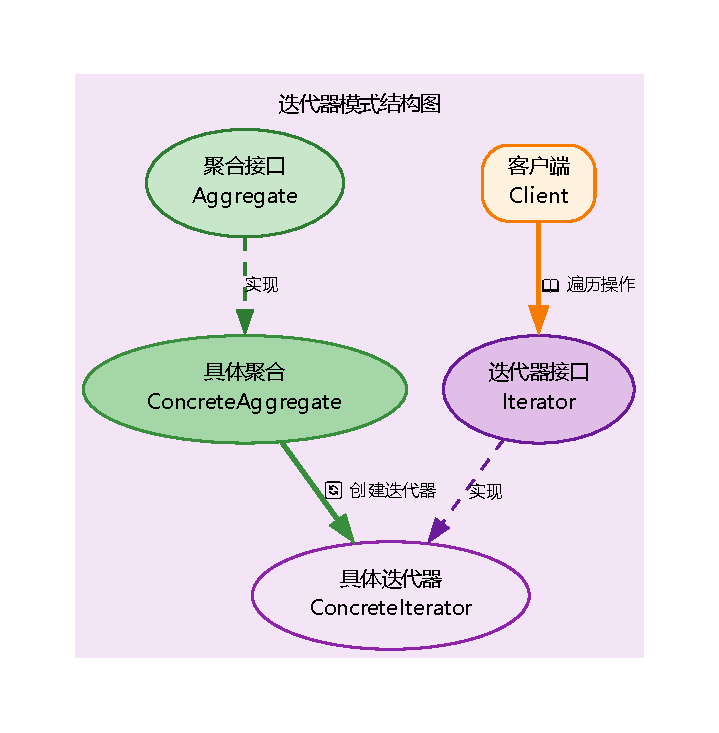
\includegraphics[width=0.9\textwidth]{images/iterator_pattern.pdf}
            \end{center}
        \end{column}
    \end{columns}
\end{frame}

\begin{frame}{迭代器模式举例说明}
    \begin{exampleytublock}{游戏背包物品遍历——统一访问不同容器}
        在一款角色扮演游戏中,玩家的背包中可能包含多种类型的物品(如武器、药水、材料等),这些物品可能分别存储在不同的数据结构中(如数组、链表、集合等)。如果客户端希望以统一的方式遍历和访问所有物品,就可以引入\textbf{迭代器模式}。其实现思路如下:
        \begin{itemize}
            \item 定义\textbf{抽象迭代器(Iterator)},规定遍历接口(如\texttt{hasNext()}、\texttt{next()}等)。
            \item 定义\textbf{具体迭代器(ConcreteIterator)},实现抽象迭代器接口,负责遍历具体的容器结构。
            \item 定义\textbf{抽象聚合(Aggregate)},声明创建迭代器的方法。
            \item 定义\textbf{具体聚合(ConcreteAggregate)},实现抽象聚合接口,返回对应的具体迭代器。
        \end{itemize}
        通过迭代器模式,客户端无需关心物品的存储结构,只需通过统一的迭代器接口即可顺序访问所有物品,极大提升了代码的灵活性和可维护性。
    \end{exampleytublock}
\end{frame}

\begin{frame}{迭代器模式示例(抽象迭代器与抽象聚合)}
    \begin{columns}
        \begin{column}{0.48\textwidth}
            \inputminted[firstline=1, lastline=14]{cpp}{code/iterator_pattern.cpp}
        \end{column}
        \begin{column}{0.48\textwidth}
            \inputminted[firstline=16, lastline=23]{cpp}{code/iterator_pattern.cpp}
        \end{column}
    \end{columns}
\end{frame}

\begin{frame}{迭代器模式示例(具体聚合)}
    \begin{columns}
        \begin{column}{0.48\textwidth}
            \inputminted[firstline=25, lastline=44]{cpp}{code/iterator_pattern.cpp}
        \end{column}
        \begin{column}{0.48\textwidth}
            \inputminted[firstline=45, lastline=61]{cpp}{code/iterator_pattern.cpp}
        \end{column}
    \end{columns}
\end{frame}

\begin{frame}{迭代器模式示例(客户端)}
    \begin{columns}
        \begin{column}{0.48\textwidth}
            \inputminted[firstline=63, lastline=68]{cpp}{code/iterator_pattern.cpp}
        \end{column}
        \begin{column}{0.48\textwidth}
            \inputminted[firstline=70, lastline=87]{cpp}{code/iterator_pattern.cpp}
        \end{column}
    \end{columns}
\end{frame}

\begin{frame}{迭代器模式优缺点}
    \begin{ytublock}{优点}
        \begin{itemize}
            \item 提供统一的遍历接口,简化客户端使用,提高代码可读性和可维护性。
            \item 支持多种遍历方式(如正序、逆序、跳跃等),灵活性较高。
            \item 可以同时遍历多个聚合对象,便于并行操作。
            \item 符合开闭原则,易于扩展新的遍历方式。
        \end{itemize}
    \end{ytublock}
    \begin{alertytublock}{缺点}
        \begin{itemize}
            \item 当聚合对象结构复杂时,迭代器的实现可能变得复杂,性能下降。
            \item 遍历过程中需要维护状态,可能导致内存消耗增加。
            \item 不支持并发访问,在多线程环境下需要额外的同步措施。
        \end{itemize}
    \end{alertytublock}
\end{frame}

\subsection{中介者模式(Mediator Pattern)}

\begin{frame}{中介者模式(Mediator Pattern)}
    通过引入一个中介对象,集中管理和协调一组对象之间的交互。
    这样,各对象之间不再直接引用彼此,降低了耦合度,使对象间的关系更清晰,交互逻辑更易于维护和扩展。

    \begin{ytublock}{适用场景}
        \begin{itemize}
            \item 系统中对象之间存在复杂的引用关系,导致依赖混乱、难以维护。
            \item 一个对象需要与许多其他对象进行通信,导致其难以复用。
            \item 希望将对象间的交互行为集中管理,避免在多个类中分散实现,减少子类数量。
        \end{itemize}
    \end{ytublock}
\end{frame}

\begin{frame}{中介者模式结构}
    \begin{columns}
        \begin{column}{0.48\textwidth}
            \begin{ytublock}{结构组成}
                \begin{itemize}
                    \item \textbf{Mediator(抽象中介者)}:定义了与各个具体同事(ConcreteColleague)通信的接口。
                    \item \textbf{ConcreteMediator(具体中介者)}:实现抽象中介者的方法,负责具体的协调工作,协调各个同事对象。
                    \item \textbf{Colleague(抽象同事)}:定义了与中介者通信的接口,同时保持与中介者的引用。
                    \item \textbf{ConcreteColleague(具体同事)}:实现抽象同事的接口,负责具体的业务逻辑,通过中介者与其他同事通信。
                \end{itemize}
            \end{ytublock}
        \end{column}
        \begin{column}{0.48\textwidth}
            \begin{center}
                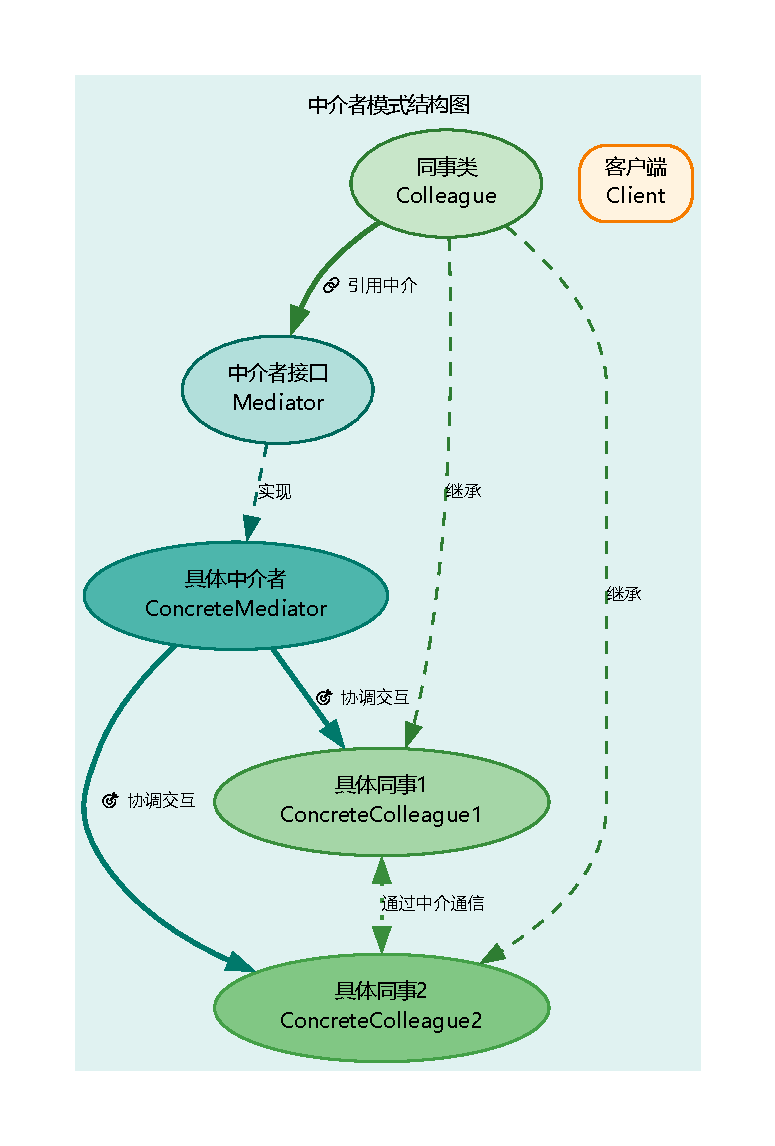
\includegraphics[width=0.7\textwidth]{images/mediator_pattern.pdf}
            \end{center}
        \end{column}
    \end{columns}
\end{frame}

\begin{frame}{中介者模式举例说明}
    \begin{exampleytublock}{多人聊天室:房间中介者集中管理玩家交互}
        假设在一个多人在线游戏中,玩家可以在同一个房间内聊天、组队、交易等。如果每个玩家对象都直接与其他所有玩家通信,系统结构会非常复杂,难以维护和扩展。\\
        为了解决这个问题,我们可以引入"房间"作为中介者。所有玩家只需与房间(中介者)通信,房间负责协调和转发消息、处理组队和交易请求等。这样,玩家之间无需直接引用彼此,极大降低了系统的耦合度。\\[0.5em]
        结构说明如下:
        \begin{itemize}
            \item \textbf{抽象中介者(Mediator)}:定义房间与玩家通信的统一接口。
            \item \textbf{具体中介者(ConcreteMediator)}:如"房间"类,实现中介者接口,负责管理和协调所有玩家的交互。
            \item \textbf{抽象同事(Colleague)}:如"玩家"基类,定义与中介者通信的接口,并持有中介者的引用。
            \item \textbf{具体同事(ConcreteColleague)}:如具体的玩家类,实现抽象同事接口,通过中介者与其他玩家间接通信,处理自身业务逻辑。
        \end{itemize}
        \textbf{总结}:通过引入房间中介者,玩家之间的交互被集中管理,系统结构更加清晰,易于维护和扩展。
    \end{exampleytublock}
\end{frame}

\begin{frame}{中介者模式示例(抽象中介者与抽象同事)}
    \begin{columns}
        \begin{column}{0.48\textwidth}
            \inputminted[firstline=1, lastline=18]{cpp}{code/mediator_pattern.cpp}
        \end{column}
        \begin{column}{0.48\textwidth}
            \inputminted[firstline=20, lastline=39]{cpp}{code/mediator_pattern.cpp}
        \end{column}
    \end{columns}
\end{frame}

\begin{frame}{中介者模式示例(具体中介者与具体同事)}
    \begin{columns}
        \begin{column}{0.48\textwidth}
            \inputminted[firstline=41, lastline=60]{cpp}{code/mediator_pattern.cpp}
        \end{column}
        \begin{column}{0.48\textwidth}
            \inputminted[firstline=62, lastline=77]{cpp}{code/mediator_pattern.cpp}
        \end{column}
    \end{columns}
\end{frame}

\begin{frame}{中介者模式示例(客户端)}
    \inputminted[firstline=86, lastline=105]{cpp}{code/mediator_pattern.cpp}
\end{frame}

\begin{frame}{中介者模式优缺点}
    \begin{ytublock}{优点}
        \begin{itemize}
            \item 集中管理对象间的交互,降低耦合度。
            \item 减少对象间的直接引用,提高系统的灵活性和可扩展性。
            \item 简化对象间的交互逻辑,使系统更易于维护。
        \end{itemize}
    \end{ytublock}
    \begin{alertytublock}{缺点}
        \begin{itemize}
            \item 中介者可能成为系统的中心化单点,增加系统的复杂性。
            \item 中介者需要处理所有对象的交互逻辑,可能导致中介者类过于庞大。
            \item 中介者模式可能引入新的依赖关系,使得系统更加复杂。
        \end{itemize}
    \end{alertytublock}
\end{frame}

\subsection{备忘录模式(Memento Pattern)}

\begin{frame}{备忘录模式(Memento Pattern)}
    在不破坏封装性的前提下,捕获并保存一个对象的内部状态,以便在需要时将其恢复到先前的状态。

    \begin{ytublock}{适用场景}
        \begin{itemize}
            \item 需要保存和恢复对象历史状态(如撤销/回退操作)。
            \item 希望避免暴露对象的实现细节,保护其封装性。
            \item 对象的状态变化较为复杂,且需要在某些时刻进行快照保存。
        \end{itemize}
    \end{ytublock}
\end{frame}

\begin{frame}{备忘录模式结构}
    \begin{ytublock}{结构组成}
        \begin{itemize}
            \item \textbf{Memento(备忘录)}:保存对象的内部状态,只能通过备忘录管理器访问。
            \item \textbf{Originator(发起者)}:创建并使用备忘录,负责创建和恢复备忘录。
            \item \textbf{Caretaker(管理者)}:负责管理备忘录,提供创建和恢复备忘录的接口。
        \end{itemize}
    \end{ytublock}
    \begin{center}
        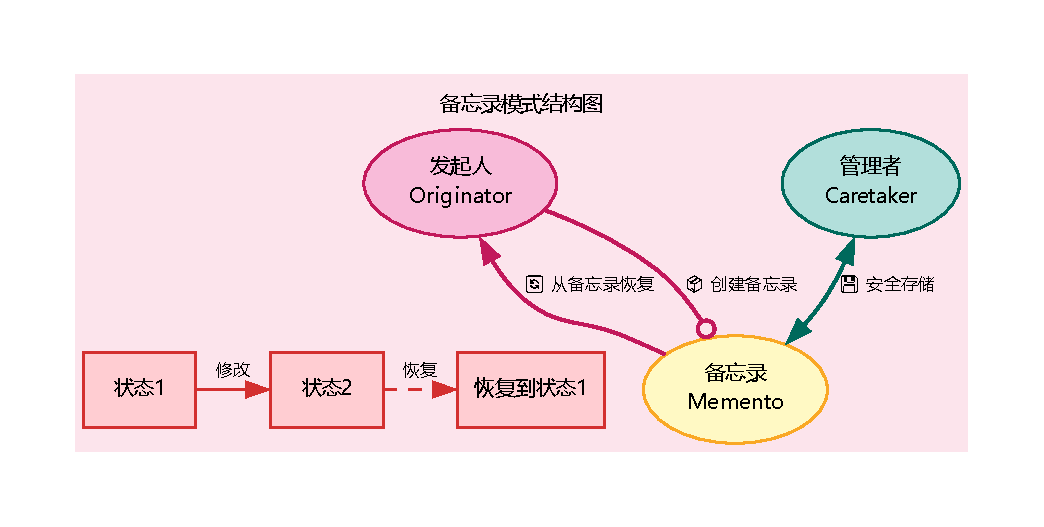
\includegraphics[width=0.7\textwidth]{images/memento_pattern.pdf}
    \end{center}
\end{frame}

\begin{frame}{备忘录模式举例说明}
    \begin{exampleytublock}{游戏进度存档——备忘录模式}
        假设我们在开发一款大型多人在线游戏,玩家可以随时保存当前的角色状态(如等级、生命、任务进度等),并在需要时恢复到某个历史存档。此时,备忘录模式可以帮助我们优雅地实现"游戏进度快照与回退"功能。其实现思路如下:
        \begin{itemize}
            \item 定义备忘录类(\texttt{Memento}),用于存储玩家的角色属性、任务进度等内部状态,外部无法直接访问其内容。
            \item 定义发起者类(\texttt{Originator}),即游戏角色本身,能够生成当前状态的备忘录,并可根据备忘录恢复到历史状态。
            \item 定义管理者类(\texttt{Caretaker}),负责保存和管理备忘录对象,实现多次撤销、重做等功能,但不会修改备忘录内容。
        \end{itemize}
    \end{exampleytublock}
\end{frame}

\begin{frame}{备忘录模式示例(备忘录)}
    \begin{columns}
        \begin{column}{0.48\textwidth}
            \inputminted[firstline=1, lastline=15]{cpp}{code/memento_pattern.cpp}
        \end{column}
        \begin{column}{0.48\textwidth}
            \inputminted[firstline=17, lastline=30]{cpp}{code/memento_pattern.cpp}
        \end{column}
    \end{columns}
\end{frame}

\begin{frame}{备忘录模式示例(发起者、管理者)}
    \begin{columns}
        \begin{column}{0.48\textwidth}
            \inputminted[firstline=17, lastline=30]{cpp}{code/memento_pattern.cpp}
        \end{column}
        \begin{column}{0.48\textwidth}
            \inputminted[firstline=32, lastline=46]{cpp}{code/memento_pattern.cpp}
        \end{column}
    \end{columns}
\end{frame}

\begin{frame}{备忘录模式示例(客户端)}
    \begin{columns}
        \begin{column}{0.48\textwidth}
            \inputminted[firstline=54, lastline=70]{cpp}{code/memento_pattern.cpp}
        \end{column}
        \begin{column}{0.48\textwidth}
            \inputminted[firstline=72, lastline=84]{cpp}{code/memento_pattern.cpp}
        \end{column}
    \end{columns}
\end{frame}

\begin{frame}{备忘录模式优缺点}
    \begin{ytublock}{优点}
        \begin{itemize}
            \item 保护了对象的封装性,避免了直接访问对象内部状态。
            \item 简化了发起者的实现,发起者只需管理备忘录的创建和恢复。
            \item 方便了管理者对备忘录的管理和维护。
        \end{itemize}
    \end{ytublock}
    \begin{alertytublock}{缺点}
        \begin{itemize}
            \item 需要额外的空间来存储备忘录,可能会占用较多的内存。
            \item 备忘录对象的创建和恢复可能会影响系统的性能和可维护性。
        \end{itemize}
    \end{alertytublock}
\end{frame}

\subsection{观察者模式(Observer Pattern)}

\begin{frame}{观察者模式(Observer Pattern)}
    观察者模式定义了一种一对多的依赖关系,使得当一个对象(被观察者/主题)的状态发生变化时,
    所有依赖于它的对象(观察者)都会自动收到通知并更新。
    \begin{ytublock}{适用场景}
        \begin{itemize}
            \item 当一个对象的改变需要同时通知并影响其他对象,且不希望这些对象之间紧密耦合时。
            \item 当系统中存在一对多的依赖关系,且被依赖方无需关心具体有多少依赖者时。
            \item 当希望对象能够动态地添加或移除依赖关系时。
        \end{itemize}
    \end{ytublock}
\end{frame}

\begin{frame}{观察者模式结构}
    \begin{columns}
        \begin{column}{0.48\textwidth}
            \begin{ytublock}{结构组成}
                \begin{itemize}
                    \item \textbf{Subject(主题/被观察者)}:定义了添加、删除观察者的方法,以及通知观察者的方法。
                    \item \textbf{ConcreteSubject(具体主题)}:实现了主题/被观察者的具体业务逻辑,当状态发生改变时,通知所有观察者。
                    \item \textbf{Observer(观察者)}:定义了更新自己的方法。
                    \item \textbf{ConcreteObserver(具体观察者)}:实现了观察者的具体业务逻辑,当收到通知时,更新自己的状态。
                \end{itemize}
            \end{ytublock}
        \end{column}
        \begin{column}{0.48\textwidth}
            \begin{center}
                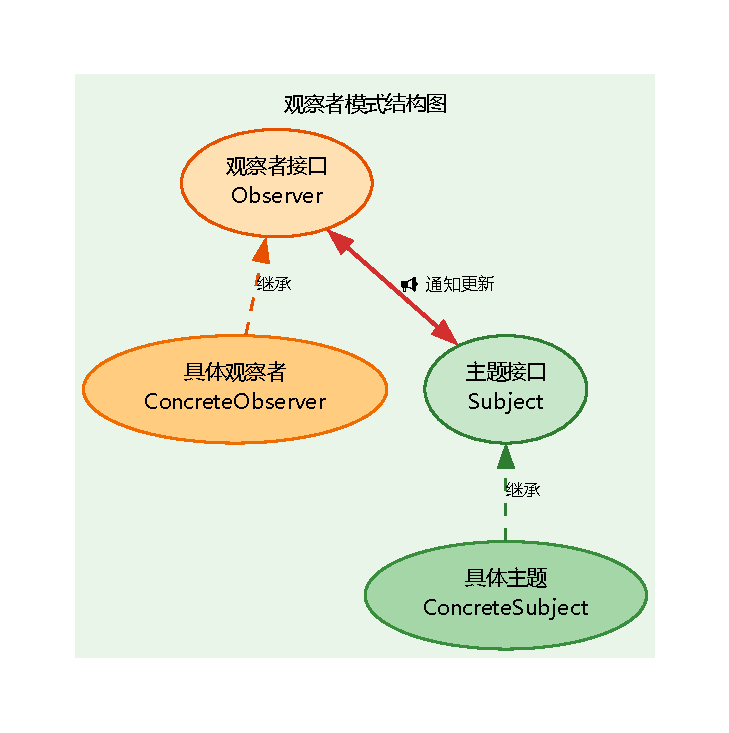
\includegraphics[width=0.9\textwidth]{images/observer_pattern.pdf}
            \end{center}
        \end{column}
    \end{columns}
\end{frame}

\begin{frame}{观察者模式举例说明}
    \begin{exampleytublock}{多人游戏任务进度通知——观察者模式}
        假设我们正在开发一款大型多人在线游戏,玩家在完成任务后需要实时通知队伍中的其他玩家当前的任务进度。此时,可以使用观察者模式来实现任务进度的自动推送和同步。其实现思路如下:
        \begin{itemize}
            \item 定义主题(\texttt{Subject}),负责维护观察者列表,并提供添加、移除和通知观察者的方法。
            \item 定义具体主题(\texttt{TaskProgress}),实现任务进度的具体业务逻辑,每当任务进度发生变化时,自动通知所有已注册的玩家。
            \item 定义观察者接口(\texttt{Observer}),声明接收通知的接口方法。
            \item 定义具体观察者(\texttt{Player}),实现接收任务进度通知的具体逻辑,玩家收到通知后可及时更新自己的界面或状态。
        \end{itemize}
    \end{exampleytublock}
\end{frame}

\begin{frame}{观察者模式示例(主题/被观察者)}
    \begin{columns}
        \begin{column}{0.48\textwidth}
            \inputminted[firstline=1, lastline=16]{cpp}{code/observer_pattern.cpp}
        \end{column}
        \begin{column}{0.48\textwidth}
            \inputminted[firstline=18, lastline=25]{cpp}{code/observer_pattern.cpp}
        \end{column}
    \end{columns}
\end{frame}

\begin{frame}{观察者模式示例(具体主题)}
    \begin{columns}
        \begin{column}{0.48\textwidth}
            \inputminted[firstline=27, lastline=44]{cpp}{code/observer_pattern.cpp}
        \end{column}
        \begin{column}{0.48\textwidth}
            \inputminted[firstline=46, lastline=57]{cpp}{code/observer_pattern.cpp}
        \end{column}
    \end{columns}
\end{frame}

\begin{frame}{观察者模式示例(具体观察者)}
    \begin{columns}
        \begin{column}{0.48\textwidth}
            \inputminted[firstline=59, lastline=70]{cpp}{code/observer_pattern.cpp}
        \end{column}
        \begin{column}{0.48\textwidth}
            \inputminted[firstline=72, lastline=84]{cpp}{code/observer_pattern.cpp}
        \end{column}
    \end{columns}
\end{frame}

\begin{frame}{观察者模式示例(客户端)}
    \begin{columns}
        \begin{column}{0.48\textwidth}
            \inputminted[firstline=90, lastline=103]{cpp}{code/observer_pattern.cpp}
        \end{column}
        \begin{column}{0.48\textwidth}
            \inputminted[firstline=105, lastline=121]{cpp}{code/observer_pattern.cpp}
        \end{column}
    \end{columns}
\end{frame}

\begin{frame}{观察者模式优缺点}
    \begin{ytublock}{优点}
        \begin{itemize}
            \item 松耦合,观察者和被观察者之间解耦,互不依赖。
            \item 易于扩展,可以动态添加或移除观察者。
        \end{itemize}
    \end{ytublock}
    \begin{alertytublock}{缺点}
        \begin{itemize}
            \item 如果观察者数量很多,通知所有观察者可能会耗费大量时间。
            \item 如果观察者之间存在循环依赖,可能会导致死循环。
        \end{itemize}
    \end{alertytublock}
\end{frame}

\subsection{策略模式(Strategy Pattern)}

\begin{frame}{策略模式(Strategy Pattern)}
    定义一系列算法,将每一个算法封装起来,并使它们可以相互替换。策略模式让算法独立于使用它的客户端而变化。

    \begin{ytublock}{适用场景}
        \begin{itemize}
            \item 系统中有许多仅在行为上有所不同的类,需要使用不同的算法或策略。
            \item 需要从多个算法中选择其一,并且可以灵活切换。
            \item 算法的实现细节对客户端隐藏,客户端无需了解具体实现。
            \item 一个类中有多种行为,并且这些行为在类的操作中以条件语句出现时,可用策略模式消除条件分支。
        \end{itemize}
    \end{ytublock}
\end{frame}

\begin{frame}{策略模式结构}
    \begin{columns}
        \begin{column}{0.48\textwidth}
            \begin{ytublock}{结构组成}
                \begin{itemize}
                    \item \textbf{Strategy(策略)}:定义了算法的接口。
                    \item \textbf{ConcreteStrategy(具体策略)}:实现了策略的接口。
                \end{itemize}
            \end{ytublock}
        \end{column}
        \begin{column}{0.48\textwidth}
            \begin{center}
                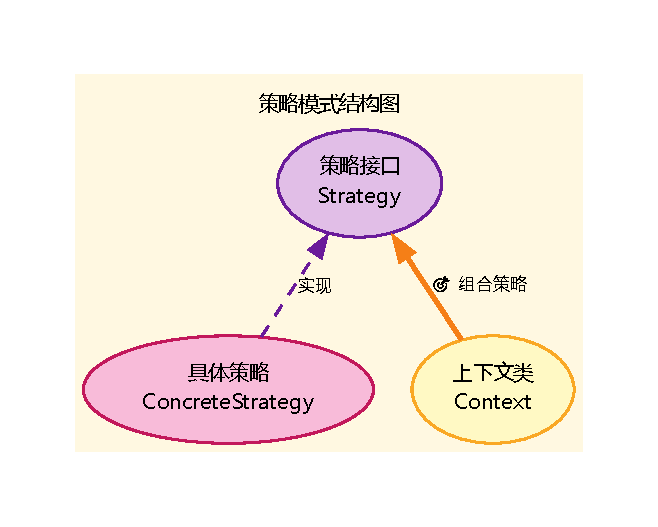
\includegraphics[width=1.0\textwidth]{images/strategy_pattern.pdf}
            \end{center}
        \end{column}
    \end{columns}
\end{frame}

\begin{frame}{策略模式举例说明}
    \begin{exampleytublock}{角色攻击方式的灵活切换}
        假设在一款游戏中,不同角色可以选择不同的攻击方式(如近战攻击、远程攻击、魔法攻击等)。每种攻击方式的实现不同,但角色可以在战斗中灵活切换攻击策略。此时可以使用\textbf{策略模式}来实现攻击方式的灵活切换,结构如下:
        \begin{itemize}
            \item 定义策略接口(\texttt{AttackStrategy}),声明攻击行为。
            \item 定义具体策略类(如\texttt{MeleeAttack}、\texttt{RangedAttack}、\texttt{MagicAttack}),实现不同的攻击方式。
            \item 角色类中持有策略接口指针,根据需要动态切换不同的攻击策略对象。
        \end{itemize}
        这样,角色无需关心具体攻击方式的实现细节,只需选择合适的策略即可完成攻击行为,极大提升了系统的灵活性和可扩展性。
    \end{exampleytublock}
\end{frame}

\begin{frame}{策略模式示例(策略)}
    \begin{columns}
        \begin{column}{0.48\textwidth}
            \inputminted[firstline=1, lastline=13]{cpp}{code/strategy_pattern.cpp}
        \end{column}
        \begin{column}{0.48\textwidth}
            \inputminted[firstline=15, lastline=24]{cpp}{code/strategy_pattern.cpp}
        \end{column}
    \end{columns}
\end{frame}

\begin{frame}{策略模式示例(具体策略)}
    \begin{columns}
        \begin{column}{0.48\textwidth}
            \inputminted[firstline=26, lastline=46]{cpp}{code/strategy_pattern.cpp}
        \end{column}
        \begin{column}{0.48\textwidth}
            \inputminted[firstline=48, lastline=68]{cpp}{code/strategy_pattern.cpp}
        \end{column}
    \end{columns}
\end{frame}

\begin{frame}{策略模式示例(客户端)}
    \inputminted[firstline=74, lastline=90]{cpp}{code/strategy_pattern.cpp}
\end{frame}

\begin{frame}{策略模式优缺点}
    \begin{ytublock}{优点}
        \begin{itemize}
            \item 灵活性,策略模式可以让算法独立于使用它的客户端而变化。
            \item 易于扩展,可以轻松添加新的策略。
        \end{itemize}
    \end{ytublock}
    \begin{alertytublock}{缺点}
        \begin{itemize}
            \item 需要为每个策略创建一个类,会增加类的数量。
            \item 客户端需要知道所有策略,并选择合适的策略。
        \end{itemize}
    \end{alertytublock}
\end{frame}

\subsection{模板方法模式(Template Method Pattern)}

\begin{frame}{模板方法模式(Template Method Pattern)}
    \textbf{模板方法模式}是一种行为型设计模式,它在父类中定义算法的整体结构(即"模板方法"),并将部分步骤的实现延迟到子类。
    这样,子类可以在不改变算法整体流程的情况下,重新定义某些特定步骤的实现。

    \begin{ytublock}{适用场景}
        \begin{itemize}
            \item 需要复用算法的整体结构,但允许部分步骤有不同实现时。
            \item 希望将多个子类中的重复代码上移到父类,减少代码冗余。
            \item 需要对子类的扩展进行统一约束和控制,防止子类破坏算法结构。
        \end{itemize}
    \end{ytublock}
\end{frame}

\begin{frame}{模板方法模式结构}
    \begin{columns}
        \begin{column}{0.38\textwidth}
            \begin{ytublock}{结构组成}
                \begin{itemize}
                    \item \textbf{抽象类(AbstractClass)}:定义算法的整体流程(模板方法),并声明若干抽象步骤。
                    \item \textbf{模板方法(Template Method)}:在抽象类中实现,规定算法的执行顺序,调用若干基本操作(可为抽象或具体)。
                    \item \textbf{具体类(ConcreteClass)}:继承抽象类,实现其中的抽象步骤,完成具体逻辑。
                \end{itemize}
            \end{ytublock}
        \end{column}
        \begin{column}{0.58\textwidth}
            \begin{center}
                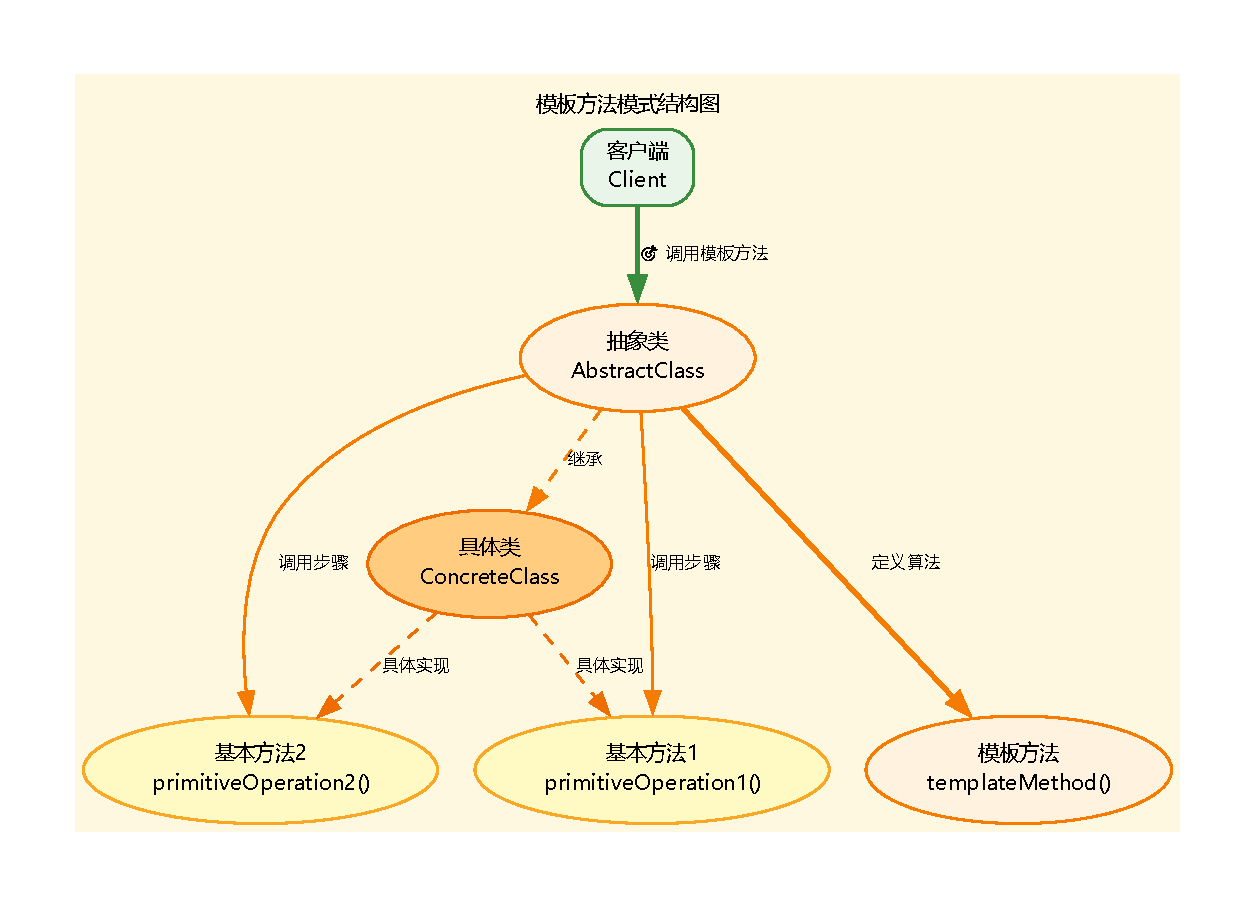
\includegraphics[width=1.0\textwidth]{images/template_method_pattern.pdf}
            \end{center}
        \end{column}
    \end{columns}
\end{frame}

\begin{frame}{模板方法模式举例说明}
    \begin{exampleytublock}{游戏中的模板方法模式——角色升级流程}
        在一款游戏中,角色升级通常需要经历多个步骤(如打怪、完成任务、收集材料等)。
        虽然每个步骤的具体实现可能不同,但升级的整体流程是固定的。
        此时可以采用\textbf{模板方法模式},将升级流程的骨架抽象出来,具体步骤由子类实现,其实现思路如下:
        \begin{itemize}
            \item 定义抽象类(\texttt{CharacterLevelUpProcess}),定义升级流程的模板方法,规定各步骤的执行顺序。
            \item 定义具体子类(\texttt{WarriorLevelUp}、\texttt{MageLevelUp}),实现抽象类中的具体步骤(如打怪、完成任务等)。
            \item 通过模板方法,保证升级流程统一,便于扩展和维护不同职业的升级细节。
        \end{itemize}
    \end{exampleytublock}
\end{frame}

\begin{frame}{模板方法模式示例(抽象类)}
    \begin{columns}
        \begin{column}{0.48\textwidth}
            \inputminted[firstline=6, lastline=24]{cpp}{code/template_method_pattern.cpp}
        \end{column}
        \begin{column}{0.48\textwidth}
            \inputminted[firstline=26, lastline=41]{cpp}{code/template_method_pattern.cpp}
        \end{column}
    \end{columns}
\end{frame}

\begin{frame}{模板方法模式示例(具体类)}
    \begin{columns}
        \begin{column}{0.48\textwidth}
            \inputminted[firstline=43, lastline=58]{cpp}{code/template_method_pattern.cpp}
        \end{column}
        \begin{column}{0.48\textwidth}
            \inputminted[firstline=60, lastline=73]{cpp}{code/template_method_pattern.cpp}
        \end{column}
    \end{columns}
\end{frame}

\begin{frame}{模板方法模式示例(客户端)}
    \inputminted[firstline=79, lastline=94]{cpp}{code/template_method_pattern.cpp}
\end{frame}

\begin{frame}{模板方法模式优缺点}
    \begin{ytublock}{优点}
        \begin{itemize}
            \item 提高代码复用性,模板方法模式将算法的通用部分抽象出来,避免重复代码。
            \item 提高代码可维护性,模板方法模式将算法的具体实现细节封装在子类中,易于维护和扩展。
        \end{itemize}
    \end{ytublock}
    \begin{alertytublock}{缺点}
        \begin{itemize}
            \item 需要为每个子类创建一个具体的实现类,增加了类的数量。
            \item 模板方法模式限制了子类的灵活性,子类必须遵守父类的模板方法。
        \end{itemize}
    \end{alertytublock}
\end{frame}

\subsection{访问者模式(Visitor Pattern)}

\begin{frame}{访问者模式(Visitor Pattern)}
    访问者模式用于将作用于对象结构中各元素的操作与元素本身进行解耦。
    通过在不修改元素类的前提下,为其添加新的操作,增强系统的扩展性和灵活性。

    \begin{ytublock}{适用场景}
        \begin{itemize}
            \item 对象结构包含多种类型的元素,需要对不同类型元素执行不同的操作。
            \item 需要在不修改元素类的情况下,为其添加新的操作,且这些操作经常变化。
            \item 希望将数据结构与操作解耦,避免操作"污染"元素类,便于维护和扩展。
            \item 元素类结构相对稳定,但对其操作需求经常变化。
        \end{itemize}
    \end{ytublock}
\end{frame}

\begin{frame}{访问者模式结构}
    \begin{columns}
        \begin{column}{0.38\textwidth}
            \begin{ytublock}{结构组成}
                \begin{itemize}
                    \item \textbf{抽象访问者(Visitor)}:定义了对各个元素的操作接口。
                    \item \textbf{具体访问者(ConcreteVisitor)}:实现抽象访问者接口,提供具体的操作实现。
                    \item \textbf{抽象元素(Element)}:定义了接受访问者的接口。
                    \item \textbf{具体元素(ConcreteElement)}:实现抽象元素接口,提供具体的操作实现。
                    \item \textbf{对象结构(ObjectStructure)}:包含多个元素,提供遍历和管理元素的方法。
                \end{itemize}
            \end{ytublock}
        \end{column}
        \begin{column}{0.58\textwidth}
            \begin{center}
                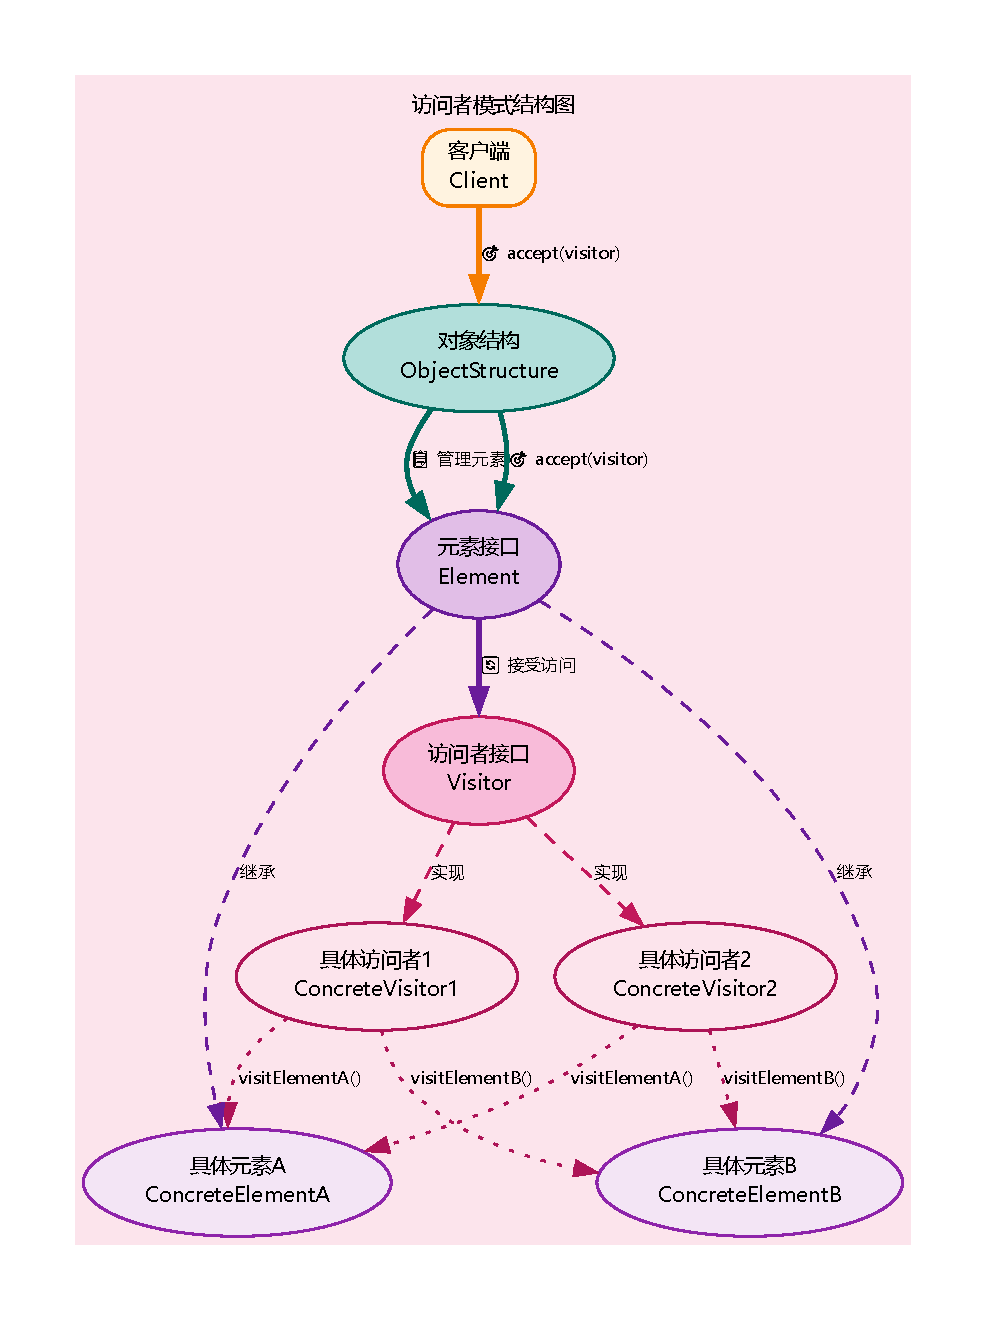
\includegraphics[width=0.8\textwidth]{images/visitor_pattern.pdf}
            \end{center}
        \end{column}
    \end{columns}
\end{frame}

\begin{frame}{访问者模式举例说明}
    \begin{exampleytublock}{RPG游戏中的访问者模式应用}
        在RPG游戏开发中,常常需要对不同类型的角色(如战士、法师、游侠等)执行多种操作(如显示状态、计算战斗力、发放奖励等)。如果将这些操作直接写在角色类中,会导致角色类臃肿且难以扩展。此时,\textbf{访问者模式}可以很好地将操作与角色类型解耦,提升系统的可扩展性和灵活性。实现思路如下:
        \begin{itemize}
            \item 定义\textbf{抽象访问者}(\texttt{Visitor}),声明针对不同角色类型的访问接口。
            \item 定义\textbf{具体访问者}(如\texttt{StatusVisitor}、\texttt{RewardVisitor}),实现具体的操作逻辑。
            \item 定义\textbf{抽象元素}(\texttt{GameCharacter}),声明接受访问者的接口(\texttt{accept}方法)。
            \item 定义\textbf{具体元素}(\texttt{Warrior}、\texttt{Mage}、\texttt{Ranger}),实现\texttt{accept}方法,并在其中调用访问者的对应方法。
            \item 定义\textbf{对象结构}(\texttt{Party}),用于管理和遍历多个角色,统一接受访问者操作。
        \end{itemize}
        通过访问者模式,可以在不修改角色类的情况下,灵活地为其添加新的操作,符合开闭原则。
    \end{exampleytublock}
\end{frame}

\begin{frame}{访问者模式示例(抽象访问者)}
    \begin{columns}
        \begin{column}{0.48\textwidth}
            \inputminted[firstline=1, lastline=20]{cpp}{code/visitor_pattern.cpp}
        \end{column}
        \begin{column}{0.48\textwidth}
            \inputminted[firstline=22, lastline=28]{cpp}{code/visitor_pattern.cpp}
        \end{column}
    \end{columns}
\end{frame}

\begin{frame}{访问者模式示例(具体访问者)}
    \begin{columns}
        \begin{column}{0.48\textwidth}
            \inputminted[firstline=30, lastline=43]{cpp}{code/visitor_pattern.cpp}
        \end{column}
        \begin{column}{0.48\textwidth}
            \inputminted[firstline=45, lastline=58]{cpp}{code/visitor_pattern.cpp}
        \end{column}
    \end{columns}
\end{frame}

\begin{frame}{访问者模式示例(具体访问者)}
    \begin{columns}
        \begin{column}{0.48\textwidth}
            \inputminted[firstline=60, lastline=73]{cpp}{code/visitor_pattern.cpp}
        \end{column}
        \begin{column}{0.48\textwidth}
            \inputminted[firstline=75, lastline=87]{cpp}{code/visitor_pattern.cpp}
        \end{column}
    \end{columns}
\end{frame}

\begin{frame}{访问者模式示例(具体访问者)}
    \begin{columns}
        \begin{column}{0.48\textwidth}
            \inputminted[firstline=89, lastline=101]{cpp}{code/visitor_pattern.cpp}
        \end{column}
        \begin{column}{0.48\textwidth}
            \inputminted[firstline=103, lastline=118]{cpp}{code/visitor_pattern.cpp}
        \end{column}
    \end{columns}
\end{frame}

\begin{frame}{访问者模式示例(客户端)}
    \begin{columns}
        \begin{column}{0.48\textwidth}
            \inputminted[firstline=120, lastline=132]{cpp}{code/visitor_pattern.cpp}
        \end{column}
        \begin{column}{0.48\textwidth}
            \inputminted[firstline=138, lastline=157]{cpp}{code/visitor_pattern.cpp}
        \end{column}
    \end{columns}
\end{frame}

\begin{frame}{访问者模式优缺点}
    \begin{ytublock}{优点}
        \begin{itemize}
            \item 将操作与数据结构分离,符合开闭原则。
            \item 可以灵活地添加新的操作,而不需要修改元素类。
        \end{itemize}
    \end{ytublock}
    \begin{alertytublock}{缺点}
        \begin{itemize}
            \item 需要为每个元素类型创建一个具体的访问者类,增加了系统的复杂性。
            \item 需要客户端知道具体的访问者类,增加了耦合度。
        \end{itemize}
    \end{alertytublock}
\end{frame}

\subsection{命令模式(Command Pattern)}

\begin{frame}{命令模式(Command Pattern)}
    命令模式将请求封装为独立的对象,允许请求的参数化、排队和撤销,提高系统的灵活性和可扩展性。
    通过将请求对象化,可以更方便地实现撤销、重做、日志记录等功能,并且支持将请求与执行操作解耦,便于扩展新的命令类型。

    \begin{ytublock}{适用场景}
        \begin{itemize}
            \item 需要将请求封装为独立的对象,以便进行参数化、排队、撤销和日志记录等操作。
            \item 需要支持撤销操作,如撤销重做、保存和恢复操作等。
            \item 需要支持修改日志,以便在系统崩溃时恢复修改。
            \item 需要将请求与执行操作解耦,便于扩展新的命令类型。
        \end{itemize}
    \end{ytublock}
\end{frame}

\begin{frame}{命令模式结构}
    \begin{columns}
        \begin{column}{0.38\textwidth}
            \begin{ytublock}{结构组成}
                \begin{itemize}
                    \item \textbf{抽象命令(Command)}:定义了执行操作的接口。
                    \item \textbf{具体命令(ConcreteCommand)}:实现抽象命令接口,定义具体的执行操作。
                    \item \textbf{接收者(Receiver)}:包含具体的业务逻辑。
                    \item \textbf{请求者(Invoker)}:负责调用命令对象执行请求。
                \end{itemize}
            \end{ytublock}
        \end{column}
        \begin{column}{0.58\textwidth}
            \begin{center}
                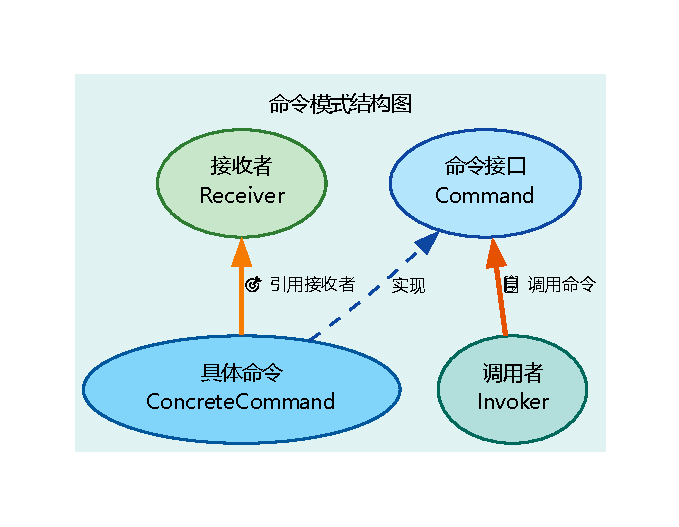
\includegraphics[width=1.0\textwidth]{images/command_pattern.pdf}
            \end{center}
        \end{column}
    \end{columns}
\end{frame}

\begin{frame}{命令模式举例说明}
    \begin{exampleytublock}{RPG游戏中的命令模式应用}
        在RPG游戏开发中,命令模式可以用于封装玩家的各种操作(如移动、攻击、使用技能等),实现操作的记录、撤销与重做、宏命令等功能。实现思路如下:
        \begin{itemize}
            \item 定义\textbf{抽象命令}(\texttt{Command}),声明执行操作的接口。
            \item 定义\textbf{具体命令}(如\texttt{MoveCommand}、\texttt{AttackCommand}、\texttt{SkillCommand}),实现具体的操作逻辑。
            \item 定义\textbf{接收者}(\texttt{Player}),包含实际的业务逻辑(如移动、攻击等方法)。
            \item 定义\textbf{请求者}(\texttt{Invoker}),负责调用命令对象执行请求,并可实现命令的撤销、重做等功能。
            \item 支持\textbf{宏命令}(\texttt{MacroCommand}),将一系列命令组合成一个复合命令,实现一键连招等功能。
        \end{itemize}
        通过命令模式,可以灵活地管理和扩展玩家操作,便于实现操作日志、回放、撤销/重做等高级功能,提升系统的可维护性和扩展性。
    \end{exampleytublock}
\end{frame}

\begin{frame}{命令模式示例(抽象命令)}
    \begin{columns}
        \begin{column}{0.48\textwidth}
            \inputminted[firstline=1, lastline=21]{cpp}{code/command_pattern.cpp}
        \end{column}
        \begin{column}{0.48\textwidth}
            \inputminted[firstline=23, lastline=40]{cpp}{code/command_pattern.cpp}
        \end{column}
    \end{columns}
\end{frame}

\begin{frame}{命令模式示例(具体命令)}
    \begin{columns}
        \begin{column}{0.48\textwidth}
            \inputminted[firstline=42, lastline=60]{cpp}{code/command_pattern.cpp}
        \end{column}
        \begin{column}{0.48\textwidth}
            \inputminted[firstline=61, lastline=80]{cpp}{code/command_pattern.cpp}
        \end{column}
    \end{columns}
\end{frame}

\begin{frame}{命令模式示例(具体命令)}
    \begin{columns}
        \begin{column}{0.48\textwidth}
            \inputminted[firstline=82, lastline=100]{cpp}{code/command_pattern.cpp}
        \end{column}
        \begin{column}{0.48\textwidth}
            \inputminted[firstline=101, lastline=120]{cpp}{code/command_pattern.cpp}
        \end{column}
    \end{columns}
\end{frame}

\begin{frame}{命令模式示例(请求者)}
    \begin{columns}
        \begin{column}{0.48\textwidth}
            \inputminted[firstline=122, lastline=127]{cpp}{code/command_pattern.cpp}
        \end{column}
        \begin{column}{0.48\textwidth}
            \inputminted[firstline=129, lastline=147]{cpp}{code/command_pattern.cpp}
        \end{column}
    \end{columns}
\end{frame}

\begin{frame}{命令模式示例(客户端)}
    \begin{columns}
        \begin{column}{0.48\textwidth}
            \inputminted[firstline=153, lastline=172]{cpp}{code/command_pattern.cpp}
        \end{column}
        \begin{column}{0.48\textwidth}
            \inputminted[firstline=173, lastline=188]{cpp}{code/command_pattern.cpp}
        \end{column}
    \end{columns}
\end{frame}

\begin{frame}{命令模式优缺点}
    \begin{ytublock}{优点}
        \begin{itemize}
            \item 将请求封装为独立的对象,方便参数化、排队、撤销和日志记录等操作。
            \item 支持撤销操作,如撤销重做、保存和恢复操作等。
            \item 支持修改日志,以便在系统崩溃时恢复修改。
            \item 将请求与执行操作解耦,便于扩展新的命令类型。
        \end{itemize}
    \end{ytublock}
    \begin{alertytublock}{缺点}
        \begin{itemize}
            \item 需要为每个命令类型创建一个具体的命令类,增加了系统的复杂性。
            \item 需要客户端知道具体的命令类,增加了耦合度。
        \end{itemize}
    \end{alertytublock}
\end{frame}

\subsection{状态模式(State Pattern)}

\begin{frame}{状态模式(State Pattern)}
    状态模式允许一个对象在其内部状态发生变化时,自动切换其行为,使得看起来像是修改了其类。
    通过将与状态相关的行为封装到独立的状态类中,状态模式实现了状态与行为的解耦,提升了系统的灵活性和可维护性。

    \begin{ytublock}{适用场景}
        \begin{itemize}
            \item 对象的行为依赖于其内部状态,并且在运行时需要根据状态切换行为。
            \item 代码中存在大量基于状态的条件分支(如if/else或switch),希望通过消除这些分支来优化结构。
            \item 需要将与状态相关的行为局部化到独立的状态类中,避免状态逻辑分散在主类中。
        \end{itemize}
    \end{ytublock}
\end{frame}

\begin{frame}{状态模式结构}
    \begin{columns}
        \begin{column}{0.48\textwidth}
            \begin{ytublock}{结构组成}
                \begin{itemize}
                    \item \textbf{抽象状态(State)}:定义了状态的接口。
                    \item \textbf{具体状态(ConcreteState)}:实现了抽象状态接口,定义了具体的状态行为。
                    \item \textbf{上下文(Context)}:包含状态的引用,并负责状态的切换。
                \end{itemize}
            \end{ytublock}
        \end{column}
        \begin{column}{0.48\textwidth}
            \begin{center}
                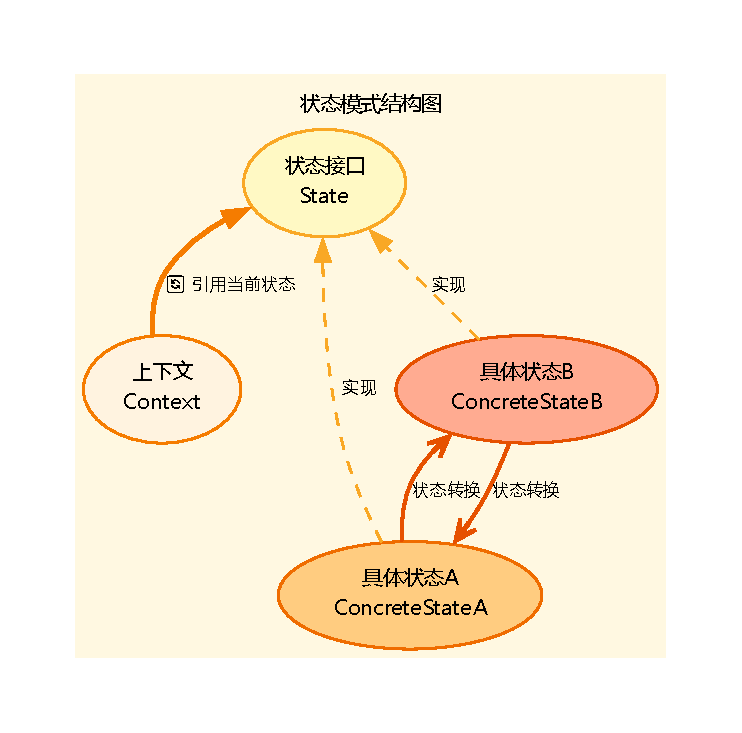
\includegraphics[width=1.0\textwidth]{images/state_pattern.pdf}
            \end{center}
        \end{column}
    \end{columns}
\end{frame}

\begin{frame}{状态模式举例说明}
    \begin{exampleytublock}{RPG游戏中的状态模式应用}
        在RPG游戏开发中,角色的行为通常取决于其当前状态(如正常、中毒、眩晕等)。如果将所有状态相关的逻辑直接堆叠在角色类中,会导致代码臃肿、难以维护和扩展。状态模式通过将每种状态的行为封装到独立的状态类中,实现了状态与行为的彻底解耦,大幅提升了系统的灵活性和可维护性。其核心实现思路如下:
        \begin{itemize}
            \item 定义\textbf{抽象状态}(\texttt{State}),统一声明所有状态应实现的接口。
            \item 定义\textbf{具体状态}(如\texttt{NormalState}、\texttt{PoisonedState}、\texttt{StunnedState}等),分别实现不同状态下的具体行为。
            \item 定义\textbf{上下文}(\texttt{CharacterContext}),持有当前状态的指针,并负责状态的切换与行为的委托。
        \end{itemize}
    \end{exampleytublock}
\end{frame}

\begin{frame}{状态模式示例(抽象状态)}
    \begin{columns}
        \begin{column}{0.48\textwidth}
            \inputminted[firstline=1, lastline=13]{cpp}{code/state_pattern.cpp}
        \end{column}
        \begin{column}{0.48\textwidth}
            \inputminted[firstline=15, lastline=24]{cpp}{code/state_pattern.cpp}
        \end{column}
    \end{columns}
\end{frame}

\begin{frame}{状态模式示例(具体状态)}
    \begin{columns}
        \begin{column}{0.48\textwidth}
            \inputminted[firstline=26, lastline=35]{cpp}{code/state_pattern.cpp}
        \end{column}
        \begin{column}{0.48\textwidth}
            \inputminted[firstline=37, lastline=46]{cpp}{code/state_pattern.cpp}
        \end{column}
    \end{columns}
\end{frame}

\begin{frame}{状态模式示例(上下文)}
    \begin{columns}
        \begin{column}{0.48\textwidth}
            \inputminted[firstline=48, lastline=62]{cpp}{code/state_pattern.cpp}
        \end{column}
        \begin{column}{0.48\textwidth}
            \inputminted[firstline=64, lastline=75]{cpp}{code/state_pattern.cpp}
        \end{column}
    \end{columns}
\end{frame}

\begin{frame}{状态模式示例(客户端)}
    \inputminted[firstline=82, lastline=101]{cpp}{code/state_pattern.cpp}
\end{frame}

\begin{frame}{状态模式优缺点}
    \begin{ytublock}{优点}
        \begin{itemize}
            \item 将每种状态的行为封装到独立的状态类中,便于扩展和维护。
            \item 状态与上下文对象解耦,状态切换灵活,代码结构清晰,易于理解和管理。
            \item 新增或修改状态时,无需修改上下文代码,降低了维护成本。
        \end{itemize}
    \end{ytublock}
    \begin{alertytublock}{缺点}
        \begin{itemize}
            \item 状态类数量随状态种类增加而增多,可能导致类爆炸,管理难度提升。
            \item 某些情况下,状态切换逻辑分散在各状态类中,可能导致切换流程不够集中,维护复杂度上升。
            \item 如果状态之间存在较多交互,可能引入额外的耦合和实现难度。
        \end{itemize}
    \end{alertytublock}
\end{frame}

\section{SOLID原则}
\begin{frame}{目录}
    \begin{multicols}{2}
        \tableofcontents[currentsection,hideothersubsections]
    \end{multicols}
\end{frame}

\subsection{SOLID原则概述}

\begin{frame}{SOLID原则简介}
    \begin{ytublock}{什么是SOLID原则?}
        SOLID是面向对象设计和编程的五个基本原则的首字母缩写:
        \begin{itemize}
            \item \textbf{S} - Single Responsibility Principle (单一职责原则)
            \item \textbf{O} - Open/Closed Principle (开闭原则)
            \item \textbf{L} - Liskov Substitution Principle (里氏替换原则)
            \item \textbf{I} - Interface Segregation Principle (接口隔离原则)
            \item \textbf{D} - Dependency Inversion Principle (依赖倒置原则)
        \end{itemize}
    \end{ytublock}

    \begin{alertytublock}{SOLID原则的重要性}
        \begin{itemize}
            \item 提高代码的可读性和可维护性
            \item 降低代码的耦合度
            \item 增强代码的灵活性和扩展性
            \item 促进代码的重用
        \end{itemize}
    \end{alertytublock}
\end{frame}

\subsection{单一职责原则 (SRP)}

\begin{frame}{单一职责原则 (SRP)}
    \begin{ytublock}{原则定义}
        \textbf{一个类应该只有一个引起它变化的原因。}
        一个类只负责一项职责,即一个类只做一件事。
        如果一个类承担的职责过多,当某一职责发生变化时,可能会影响到其他职责的实现,导致代码难以维护和扩展。
    \end{ytublock}
    \begin{ytublock}{SRP的优势}
        \begin{itemize}
            \item 提高代码的可维护性:每个类只负责一项职责,代码结构清晰,便于理解和维护。
            \item 降低变更带来的风险:当某一职责发生变化时,只需修改对应的类,不会影响到其他无关的功能。
            \item 便于代码复用:职责单一的类更容易被复用到其他场景中。
            \item 促进团队协作:不同开发人员可以专注于不同的类或模块,减少冲突,提高开发效率。
            \item 有助于单元测试:单一职责的类更容易编写针对性的测试用例,提高测试覆盖率和准确性。
        \end{itemize}

    \end{ytublock}
\end{frame}

\begin{frame}{单一职责原则(SRP)示例}
    \begin{exampleytublock}{设计模式案例:抽象工厂模式中的职责分离}
        以\textbf{抽象工厂模式(Abstract Factory Pattern)}为例,假设我们要开发一个奶茶店系统。系统中有奶茶(如\texttt{Tea})和配料(如\texttt{Topping})两大类产品。每个产品族(如原味、甜味、巧克力味)都需要生产一组相关的奶茶和配料。<br>
        在抽象工厂模式中,\texttt{Tea}和\texttt{Topping}分别作为独立的抽象产品类,各自只负责自身的属性和行为;\texttt{TeaFactory}作为抽象工厂,只负责定义创建奶茶和配料的接口;每个具体工厂(如\texttt{OriginalFactory}、\texttt{SweetFactory}、\texttt{ChocolateFactory})只负责生产一组特定口味的奶茶和配料。<br>
        这样,每个类都只承担单一职责:产品类只关注产品本身,工厂类只关注产品的创建,产品族的扩展和维护都非常清晰,充分体现了单一职责原则。
    \end{exampleytublock}
\end{frame}

\begin{frame}{单一职责原则(SRP)示例}
    \begin{alertytublock}{不遵循SRP的后果(以抽象工厂模式为例)}
        \begin{itemize}
            \item \textbf{代码难以维护:} 如果将所有奶茶和配料的创建逻辑都写在一个大工厂类或产品类中,添加或修改产品时需要频繁修改同一个类,容易引入bug。
            \item \textbf{可读性和可测试性降低:} 产品类既包含自身属性又包含其他产品或配料的逻辑,代码臃肿,难以理解和测试。
            \item \textbf{复用性差:} 其他饮品或配料想要复用某种创建逻辑,必须复制粘贴相关代码,无法灵活组合。
            \item \textbf{团队协作受阻:} 多人同时修改同一个大类时,容易产生冲突,影响开发效率。
            \item \textbf{扩展性受限:} 新增产品族或变更产品逻辑时,必须修改已有类,系统演化困难。
        \end{itemize}
    \end{alertytublock}
\end{frame}

\begin{frame}{SRP与设计模式}
    \begin{ytublock}{SRP在设计模式中的体现}
        \begin{itemize}
            \item \textbf{策略模式(Strategy Pattern):} 将可变的算法行为抽象为独立的策略类,每个策略类只负责一种算法,便于扩展和维护,避免算法混杂在主业务类中。
            \item \textbf{命令模式(Command Pattern):} 将请求的每个操作封装为独立的命令对象,每个命令类只负责一种具体操作,调用者与执行者解耦,便于扩展新命令。
            \item \textbf{工厂模式(Factory Pattern):} 将对象的创建逻辑集中到工厂类中,产品类只关注自身职责,工厂类只负责对象的实例化,职责分明。
            \item \textbf{装饰器模式(Decorator Pattern):} 将附加功能封装到装饰器类中,核心组件类只关注核心职责,装饰器类只负责扩展功能,二者职责清晰。
            \item \textbf{观察者模式(Observer Pattern):} 主题对象只负责自身状态的维护,观察者对象只负责响应状态变化,二者各司其职,便于独立演化。
            \item \textbf{状态模式(State Pattern):} 每个状态类只负责一种状态下的行为,状态切换逻辑与具体行为分离,便于扩展新状态。
        \end{itemize}
    \end{ytublock}
\end{frame}

\subsection{开闭原则 (OCP)}

\begin{frame}{开闭原则 (OCP)}
    \begin{ytublock}{原则定义}
        \textbf{软件实体(类、模块、函数等)应该对扩展开放,对修改关闭。}
        这意味着在添加新功能时,不应修改现有代码,而是通过扩展来实现。
    \end{ytublock}
    \begin{ytublock}{OCP的优势}
        \begin{itemize}
            \item 提高系统的可扩展性:容易添加新功能而不影响现有代码。
            \item 降低风险:修改现有代码可能引入bug,扩展则更安全。
            \item 促进代码复用:现有代码保持稳定,可被新扩展复用。
            \item 便于测试:新功能可独立测试,不干扰原有系统。
            \item 支持持续集成:新扩展可无缝融入现有系统。
        \end{itemize}
    \end{ytublock}
\end{frame}

\begin{frame}{开闭原则(OCP)示例}
    \begin{exampleytublock}{现实案例:策略模式下的攻击方式扩展}
        以\textbf{策略模式(Strategy Pattern)}为例,假设在一款游戏中,角色可以选择不同的攻击方式(如近战攻击、远程攻击、魔法攻击等)。<br>
        如果采用传统实现,角色类中可能通过大量\texttt{if-else}或\texttt{switch}语句判断攻击类型,每增加一种新攻击方式都需要修改角色类的代码,容易引入bug,违背开闭原则。<br>
        使用策略模式后,每种攻击方式都实现统一的\texttt{AttackStrategy}接口,角色类只依赖该接口。<br>
        当需要扩展新的攻击方式时,只需新增一个策略类实现\texttt{AttackStrategy},无需修改角色类的任何代码。<br>
        这正体现了开闭原则:系统对新功能(新攻击方式)的扩展开放,对已有代码的修改关闭,保证了系统的稳定性和可维护性。
    \end{exampleytublock}
\end{frame}

\begin{frame}{开闭原则(OCP)示例}
    \begin{alertytublock}{不遵循OCP的后果(以策略模式为例)}
        \begin{itemize}
            \item \textbf{代码脆弱性增加:} 每次添加新攻击方式都要修改角色类,容易引入新bug或破坏原有功能。
            \item \textbf{维护成本上升:} 修改核心角色类可能导致连锁反应,需要大量回归测试,消耗时间和资源。
            \item \textbf{可扩展性受限:} 系统变得僵化,添加新攻击方式的风险高,导致开发效率低下。
            \item \textbf{版本控制复杂:} 频繁修改角色类增加合并冲突的风险,影响团队协作。
            \item \textbf{系统稳定性下降:} 积累的修改可能使代码难以理解和预测,增加出错概率。
        \end{itemize}
    \end{alertytublock}
\end{frame}

\begin{frame}{OCP与设计模式}
    \begin{ytublock}{OCP在设计模式中的体现}
        \begin{itemize}
            \item \textbf{策略模式(Strategy Pattern):} 通过定义算法族并封装每个算法,允许在运行时切换算法,实现对扩展开放。
            \item \textbf{装饰器模式(Decorator Pattern):} 动态地为对象添加新行为,而不修改其结构,支持功能扩展。
            \item \textbf{工厂模式(Factory Pattern):} 通过子类决定实例化哪个类,实现对新类型的扩展而不改动现有代码。
            \item \textbf{观察者模式(Observer Pattern):} 允许添加新观察者而不修改主题类,实现松耦合扩展。
            \item \textbf{模板方法模式(Template Method Pattern):} 在超类中定义算法骨架,子类重写具体步骤,实现扩展而不改动算法结构。
            \item \textbf{桥接模式(Bridge Pattern):} 将抽象与实现分离,允许两者独立变化,支持扩展。
        \end{itemize}
    \end{ytublock}
\end{frame}

\subsection{里氏替换原则 (LSP)}

\begin{frame}{里氏替换原则 (LSP)}
    \begin{ytublock}{原则定义}
        \textbf{子类对象必须能够替换掉所有父类对象,而不影响程序的正确性。}
        继承时,子类应扩展父类行为,而不应改变或限制它。
    \end{ytublock}
    \begin{ytublock}{LSP的优势}
        \begin{itemize}
            \item 确保继承关系的正确性:子类可无缝替换父类,提高代码的可靠性。
            \item 促进多态使用:安全地使用多态特性,实现灵活的代码设计。
            \item 提高可维护性:修改子类不会意外影响依赖父类的代码。
            \item 便于扩展:允许通过继承添加新功能,而不破坏现有系统。
            \item 支持开闭原则:通过子类扩展实现OCP。
        \end{itemize}
    \end{ytublock}
\end{frame}

\begin{frame}{里氏替换原则(LSP)示例}
    \begin{exampleytublock}{现实案例:模板方法模式中的角色升级}
        假设有一个抽象类\texttt{CharacterLevelUpProcess},定义了角色升级的整体流程(模板方法),并声明了若干抽象步骤(如打怪、完成任务、收集材料等)。<br>
        子类如\texttt{WarriorLevelUp}和\texttt{MageLevelUp}分别实现这些步骤,体现不同职业的升级细节。<br>
        如果某个子类在重写抽象步骤时,破坏了父类模板方法的整体流程(比如直接跳过某些关键步骤或改变流程顺序),那么用该子类对象替换父类对象时,升级流程就会出错,违反LSP。<br>
        正确做法是:子类只重写具体步骤的实现,不改变父类模板方法的结构,这样任何子类都能安全替换父类,保证升级流程的正确性。
    \end{exampleytublock}
\end{frame}

\begin{frame}{里氏替换原则(LSP)示例}
    \begin{alertytublock}{不遵循LSP的后果(以模板方法为例)}
        \begin{itemize}
            \item \textbf{多态失效:} 子类如果随意更改模板方法流程,父类引用指向子类对象时,整体算法可能被破坏,失去多态的意义。
            \item \textbf{代码不可靠:} 依赖父类流程的代码在子类替换后可能出现逻辑错误,降低系统稳定性。
            \item \textbf{维护困难:} 需要为每个子类单独检查流程正确性,增加维护和测试难度。
            \item \textbf{扩展受限:} 继承关系不安全,开发者不敢放心扩展新子类,影响系统灵活性。
            \item \textbf{测试复杂:} 需要为每个子类单独测试完整流程,增加测试负担。
        \end{itemize}
    \end{alertytublock}
\end{frame}

\begin{frame}{LSP与设计模式}
    \begin{ytublock}{LSP在设计模式中的体现}
        \begin{itemize}
            \item \textbf{模板方法模式(Template Method Pattern):} 子类重写具体步骤,但必须遵守父类的算法结构。
            \item \textbf{策略模式(Strategy Pattern):} 所有策略类实现同一接口,确保可替换性。
            \item \textbf{工厂方法模式(Factory Method Pattern):} 子工厂创建的产品必须符合产品接口。
            \item \textbf{组合模式(Composite Pattern):} 叶节点和复合节点统一接口,确保替换不影响树结构。
            \item \textbf{命令模式(Command Pattern):} 所有命令对象实现同一接口,支持替换。
            \item \textbf{状态模式(State Pattern):} 状态类实现同一接口,确保状态切换不违反LSP。
        \end{itemize}
    \end{ytublock}
\end{frame}

\subsection{接口隔离原则 (ISP)}

\begin{frame}{接口隔离原则 (ISP)}
    \begin{ytublock}{原则定义}
        \textbf{客户端不应被迫依赖于它们不使用的接口。}
        接口应细粒度设计,只包含客户端需要的功能。
    \end{ytublock}
    \begin{ytublock}{ISP的优势}
        \begin{itemize}
            \item 降低耦合:客户端只依赖所需接口,减少不必要依赖。
            \item 提高灵活性:易于修改和扩展接口而不影响无关客户端。
            \item 便于测试:小接口更容易mock和测试。
            \item 支持单一职责:接口职责单一,与SRP相辅相成。
            \item 改善可维护性:变化只影响相关客户端。
        \end{itemize}
    \end{ytublock}
\end{frame}

\begin{frame}{接口隔离原则(ISP)示例}
    \begin{exampleytublock}{现实案例:音频播放器适配器)}
        假设有一个音频播放器系统,原本只支持播放MP3格式(\texttt{Mp3Player}),现在需要支持MP4和VLC格式。<br>
        如果将所有播放方法(如\texttt{playMp3}、\texttt{playMp4}、\texttt{playVlc})都放在一个大接口\texttt{MediaPlayer}中,则即使只播放MP3的类也必须实现MP4和VLC方法(即使为空),这违反了接口隔离原则。<br>
        正确做法:将不同格式的播放功能拆分为不同接口(如\texttt{Mp3Playable}、\texttt{Mp4Playable}、\texttt{VlcPlayable}),播放器只实现自己需要的接口。<br>
        适配器模式通过组合这些小接口,实现灵活扩展和最小依赖,完美体现了ISP。
    \end{exampleytublock}
\end{frame}

\begin{frame}{接口隔离原则(ISP)示例}
    \begin{alertytublock}{不遵循ISP的后果(以适配器为例)}
        \begin{itemize}
            \item \textbf{耦合度高:} 只支持MP3的播放器也被迫实现MP4、VLC等无关方法,增加冗余代码。
            \item \textbf{灵活性差:} 新增或修改某种格式的播放方法时,所有实现大接口的类都受影响。
            \item \textbf{代码臃肿:} 播放器类中充斥大量无用或空实现的方法,降低可读性。
            \item \textbf{测试困难:} 需要为所有方法编写测试,即使某些方法实际不会被用到。
            \item \textbf{维护成本高:} 任何接口变动都可能影响所有播放器实现,容易引入bug。
        \end{itemize}
    \end{alertytublock}
\end{frame}

\begin{frame}{ISP与设计模式}
    \begin{ytublock}{ISP在设计模式中的体现}
        \begin{itemize}
            \item \textbf{适配器模式(Adapter Pattern):} 通过适配器提供最小接口,隐藏复杂实现。
            \item \textbf{外观模式(Facade Pattern):} 提供简化接口,隔离子系统复杂性。
            \item \textbf{装饰器模式(Decorator Pattern):} 每个装饰器实现特定接口,支持细粒度扩展。
            \item \textbf{代理模式(Proxy Pattern):} 代理实现与主体相同的接口,但可添加控制。
            \item \textbf{桥接模式(Bridge Pattern):} 分离抽象和实现接口,支持独立变化。
            \item \textbf{组合模式(Composite Pattern):} 统一组件接口,但允许叶节点只实现必要方法。
        \end{itemize}
    \end{ytublock}
\end{frame}

\subsection{依赖倒置原则 (DIP)}

\begin{frame}{依赖倒置原则 (DIP)}
    \begin{ytublock}{原则定义}
        \textbf{高层模块不应依赖低层模块,二者都应依赖抽象。}
        抽象不应依赖细节,细节应依赖抽象。
    \end{ytublock}
    \begin{ytublock}{DIP的优势}
        \begin{itemize}
            \item 降低耦合:通过抽象解耦高层和低层模块。
            \item 提高灵活性:易于替换实现而不影响高层。
            \item 便于测试:可使用mock实现测试高层逻辑。
            \item 支持开闭原则:通过新实现扩展功能。
            \item 促进模块化:鼓励使用接口和抽象类。
        \end{itemize}
    \end{ytublock}
\end{frame}

\begin{frame}{依赖倒置原则(DIP)示例}
    \begin{exampleytublock}{现实案例:多人游戏任务进度通知(观察者模式)}
        传统做法:任务进度类直接依赖具体玩家类,通知时需要逐个调用具体玩家的更新方法。如果玩家类型变化或增加新类型,任务进度类必须修改,导致高耦合,违背DIP。\\
        正确做法:定义\texttt{Observer}(观察者)接口,所有玩家类实现该接口。任务进度类(主题)只依赖\texttt{Observer}接口,不关心具体玩家类型。\\
        当有新玩家类型加入时,只需实现\texttt{Observer}接口,无需修改任务进度类,实现了高层(任务进度)依赖抽象,低层(玩家)依赖抽象,完美体现依赖倒置原则。
    \end{exampleytublock}
\end{frame}

\begin{frame}{依赖倒置原则(DIP)示例}
    \begin{alertytublock}{不遵循DIP的后果(以观察者模式为例)}
        \begin{itemize}
            \item \textbf{高耦合:} 任务进度类直接依赖具体玩家类,新增或修改玩家类型时需修改任务进度类。
            \item \textbf{灵活性低:} 玩家类型变化会影响任务进度类,扩展新玩家不便。
            \item \textbf{测试困难:} 任务进度类与具体玩家强耦合,难以对任务进度逻辑单独测试。
            \item \textbf{可维护性差:} 代码臃肿,维护和扩展成本高。
            \item \textbf{扩展受限:} 新增玩家类型或通知方式时,必须修改高层代码,违背OCP。
        \end{itemize}
    \end{alertytublock}
\end{frame}

\begin{frame}{DIP与设计模式}
    \begin{ytublock}{DIP在设计模式中的体现}
        \begin{itemize}
            \item \textbf{工厂模式(Factory Pattern):} 通过工厂创建对象,高层依赖抽象而非具体类。
            \item \textbf{依赖注入(Dependency Injection):} 将依赖通过构造函数或setter注入,实现倒置。
            \item \textbf{策略模式(Strategy Pattern):} 高层依赖策略接口,低层实现具体策略。
            \item \textbf{观察者模式(Observer Pattern):} 主题依赖观察者接口,具体观察者实现接口。
            \item \textbf{桥接模式(Bridge Pattern):} 抽象层依赖实现接口,支持多种实现。
            \item \textbf{命令模式(Command Pattern):} 调用者依赖命令接口,具体命令实现细节。
        \end{itemize}
    \end{ytublock}
\end{frame}

\subsection{SOLID原则总结}

\begin{frame}{SOLID原则总结}
    \begin{ytublock}{SOLID原则的相互关系}
        \begin{itemize}
            \item \textbf{SRP} 为 OCP 提供基础,确保职责单一便于扩展
            \item \textbf{OCP} 依赖 LSP,通过继承实现扩展
            \item \textbf{LSP} 是 OCP 的基础,保证继承关系的正确性
            \item \textbf{ISP} 支持 DIP,通过接口隔离实现依赖倒置
            \item \textbf{DIP} 是 OCP 的高层实现,通过抽象实现解耦
        \end{itemize}
    \end{ytublock}

    \begin{exampleytublock}{SOLID原则的应用实践}
        \begin{itemize}
            \item 在设计类和接口时首先考虑单一职责
            \item 使用抽象和接口来实现开闭原则
            \item 确保继承关系符合里氏替换原则
            \item 将大接口拆分为小接口以遵循接口隔离
            \item 通过依赖注入实现依赖倒置
        \end{itemize}
    \end{exampleytublock}
\end{frame}

\begin{frame}{SOLID原则与设计模式的关系}
    \begin{ytublock}{设计模式对SOLID原则的支持}
        SOLID原则是设计模式的基础,而设计模式则是SOLID原则的具体实现方式:
    \end{ytublock}

    \begin{columns}
        \begin{column}{0.5\textwidth}
            \begin{itemize}
                \item \textbf{策略模式} → OCP + DIP
                \item \textbf{工厂模式} → DIP + SRP
                \item \textbf{装饰器模式} → OCP + ISP
                \item \textbf{观察者模式} → OCP + DIP
                \item \textbf{适配器模式} → ISP + LSP
            \end{itemize}
        \end{column}
        \begin{column}{0.5\textwidth}
            \begin{itemize}
                \item \textbf{命令模式} → SRP + OCP
                \item \textbf{模板方法} → LSP + OCP
                \item \textbf{组合模式} → LSP + OCP
                \item \textbf{桥接模式} → OCP + DIP
                \item \textbf{外观模式} → ISP + DIP
            \end{itemize}
        \end{column}
    \end{columns}

    \begin{alertytublock}{学习建议}
        \begin{itemize}
            \item 先掌握SOLID原则,再学习设计模式
            \item 在实际项目中结合使用原则和模式
            \item 通过代码重构实践SOLID原则
            \item 编写单元测试验证原则的正确性
        \end{itemize}
    \end{alertytublock}
\end{frame}

\section{总结}
\begin{frame}{目录}
    \begin{multicols}{2}
        \tableofcontents[currentsection,hideallsubsections]
    \end{multicols}
\end{frame}

\begin{frame}{设计模式总结}
    \begin{ytublock}{23种GoF设计模式的完整总结}
        \begin{columns}
            \begin{column}{0.5\textwidth}
                \textbf{创建型模式 (5种)}
                \begin{itemize}
                    \item 单例:唯一实例,全局访问
                    \item 工厂方法:延迟创建,子类决定
                    \item 抽象工厂:产品家族,系列创建
                    \item 建造者:分步构建,复杂对象
                    \item 原型:对象克隆,复制创建
                \end{itemize}
            \end{column}
            \begin{column}{0.5\textwidth}
                \textbf{结构型模式 (7种)}
                \begin{itemize}
                    \item 适配器:接口转换,兼容性
                    \item 桥接:抽象分离,解耦合
                    \item 组合:树形结构,整体-部分
                    \item 装饰器:动态扩展,功能增强
                    \item 外观:简化接口,统一入口
                    \item 享元:对象共享,内存优化
                    \item 代理:访问控制,权限管理
                \end{itemize}
            \end{column}
        \end{columns}
    \end{ytublock}
\end{frame}

\begin{frame}{设计模式总结 (续)}
    \begin{ytublock}{行为型模式 (11种)}
        \begin{columns}
            \begin{column}{0.5\textwidth}
                \begin{itemize}
                    \item 责任链:请求传递,多级处理
                    \item 命令:请求封装,支持撤销
                    \item 解释器:语言解析,文法表示
                    \item 迭代器:顺序访问,遍历集合
                    \item 中介者:对象交互,解耦通信
                    \item 备忘录:状态保存,支持回退
                \end{itemize}
            \end{column}
            \begin{column}{0.5\textwidth}
                \begin{itemize}
                    \item 观察者:事件通知,一对多依赖
                    \item 状态:状态变迁,行为改变
                    \item 策略:算法选择,可互换
                    \item 模板方法:算法框架,子类扩展
                    \item 访问者:双重分派,操作扩展
                \end{itemize}
            \end{column}
        \end{columns}
    \end{ytublock}
\end{frame}

\begin{frame}{学习路径建议}
    \begin{ytublock}{入门级学习路径}
        \begin{enumerate}
            \item \textbf{单例模式} - 理解对象唯一性概念
            \item \textbf{工厂方法} - 掌握对象创建模式
            \item \textbf{观察者模式} - 学习事件驱动编程
            \item \textbf{策略模式} - 理解算法封装思想
        \end{enumerate}
    \end{ytublock}

    \begin{ytublock}{进阶级学习路径}
        \begin{enumerate}
            \item \textbf{装饰器模式} - 掌握对象功能扩展
            \item \textbf{组合模式} - 理解树形数据结构
            \item \textbf{命令模式} - 学习撤销重做机制
            \item \textbf{模板方法} - 掌握算法框架设计
        \end{enumerate}
    \end{ytublock}
\end{frame}

\begin{frame}{学习路径建议 (续)}
    \begin{ytublock}{高级学习路径}
        \begin{enumerate}
            \item \textbf{访问者模式} - 双重分派技术
            \item \textbf{解释器模式} - 语言处理基础
            \item \textbf{桥接模式} - 抽象与实现分离
            \item \textbf{中介者模式} - 复杂对象交互
        \end{enumerate}
    \end{ytublock}

    \begin{ytublock}{实践建议}
        \begin{itemize}
            \item 每个模式都要动手实现,加深理解
            \item 分析现有代码,识别可应用的设计模式
            \item 结合实际项目,灵活运用设计模式
            \item 持续学习,设计模式是软件开发的基石
        \end{itemize}
    \end{ytublock}
\end{frame}

\begin{frame}{设计模式的应用原则}
    \begin{ytublock}{SOLID原则与设计模式}
        \begin{itemize}
            \item \textbf{S - 单一职责原则}:每个类应该只有一个职责
            \item \textbf{O - 开闭原则}:对扩展开放,对修改关闭
            \item \textbf{L - 里氏替换原则}:子类可以替换父类
            \item \textbf{I - 接口隔离原则}:接口应该小而专一
            \item \textbf{D - 依赖倒置原则}:依赖抽象而不依赖具体
        \end{itemize}
    \end{ytublock}

    \begin{ytublock}{设计模式遵循的原则}
        \begin{itemize}
            \item 大多数设计模式都遵循SOLID原则
            \item 设计模式是这些原则的具体体现
            \item 理解原则才能更好地应用模式
            \item 原则是基础,模式是应用
        \end{itemize}
    \end{ytublock}
\end{frame}

\begin{frame}{设计模式的优势与局限性}
    \begin{columns}
        \begin{column}{0.48\textwidth}
            \begin{ytublock}{主要优势}
                \begin{itemize}
                    \item 提高代码的可复用性
                    \item 增强代码的可维护性
                    \item 促进代码的可扩展性
                    \item 降低代码的耦合度
                    \item 提高开发效率
                    \item 便于团队协作
                    \item 提升软件质量
                \end{itemize}
            \end{ytublock}
        \end{column}
        \begin{column}{0.48\textwidth}
            \begin{alertytublock}{可能的局限性}
                \begin{itemize}
                    \item 增加代码复杂度
                    \item 可能影响性能
                    \item 学习成本较高
                    \item 过度使用可能适得其反
                \end{itemize}
            \end{alertytublock}
        \end{column}
    \end{columns}
\end{frame}

\begin{frame}{如何选择合适的设计模式}
    \begin{ytublock}{选择原则}
        \begin{itemize}
            \item 根据具体问题选择最合适的设计模式
            \item 不要为了使用模式而使用模式
            \item 考虑团队成员的理解程度
            \item 权衡模式的复杂度和带来的收益
            \item 优先考虑简单有效的解决方案
        \end{itemize}
    \end{ytublock}

    \begin{ytublock}{实践建议}
        \begin{itemize}
            \item 多读优秀开源代码,学习模式应用
            \item 参与代码审查,讨论设计决策
            \item 持续学习,跟踪设计模式的新发展
            \item 在实践中检验和改进自己的理解
        \end{itemize}
    \end{ytublock}
\end{frame}

\begin{frame}{参考资料与学习资源}
    \begin{ytublock}{经典著作}
        \begin{itemize}
            \item  \textbf{《Clean Code》}
            \item 《Agile Software Development, Principles, Patterns, and Practices》
            \item 《Refactoring: Improving the Design of Existing Code》
            \item 《Clean Architecture》

            \item 《设计模式:可复用面向对象软件的基础》
            \item 《Head First设计模式》
            \item 《大话设计模式》
            \item 《设计模式之禅》
        \end{itemize}
    \end{ytublock}
\end{frame}

\begin{frame}{结语}
    \begin{center}
        \Huge{\textbf{感谢学习!}}

        \vspace{1cm}

        \Large{设计模式的学习是一个持续的过程}

        \vspace{0.5cm}

        \large{通过实践和应用,才能真正掌握这些宝贵的经验}

        \vspace{1cm}

        \textbf{祝您编程愉快!}
    \end{center}
\end{frame}

\end{document}
